% Relazione — elaborato di Tipo A, Sistemi Distribuiti (UNIFI)
% Classe: Tptesi2 (template UNIFI, incluso in questa cartella).
% Compilazione: pdflatex x2  (vedi README.md in questa cartella)
\documentclass[a4paper,oneside]{Tptesi2}

% Tptesi2 carica gia': babel(italian), inputenc, fontenc, amsmath, amssymb,
% graphicx, hyperref, float, algorithm2e, mathrsfs. Qui serve solo il resto.
\usepackage{booktabs}
% Percorsi di file lunghi che possono andare a capo (evita overflow del margine).
\usepackage{seqsplit}
\newcommand{\exfile}[1]{\texttt{\seqsplit{examples/#1.json}}}

% Le figure vivono nelle cartelle del progetto: nessuna copia duplicata.
% "figures/" viene provata per prima, cosi' e' possibile creare un progetto
% Overleaf autonomo copiando li' le immagini necessarie.
\graphicspath{{figures/}{img/}{../docs/diagrams/}{../screenshots/}}

\hypersetup{%
  plainpages=false,%
  breaklinks,%
  pdftitle={Mobility Advisor per Snap4City},%
  pdfauthor={Junliang Zheng},%
  pdfsubject={Elaborato di Tipo A - Sistemi Distribuiti},%
  colorlinks=false}

\begin{document}

\frontmatter

% ---------------------------------------------------------------------
% Frontespizio: riprende l'impaginazione del template, con la dicitura
% corretta per un elaborato (il \maketitle della classe scrive "Tesi di
% Laurea Triennale").
% ---------------------------------------------------------------------
\begin{titlepage}
  \centering
  \vspace*{-10mm}
  
\includegraphics[height=30mm]{stemma}\\[4mm]
  {\textsc{\Large Universit\`a degli Studi di Firenze}}\\[2mm]
  {\textsc{Scuola di Ingegneria --- Dipartimento di Ingegneria dell'Informazione}}\\[3mm]
  \rule{50mm}{0.01mm}\\[3mm]
  {\small Elaborato di Tipo A per il corso di}\\[1mm]
  {\large Sistemi Distribuiti}

  \vfill

  {\Large\bfseries\textsc{Mobility Advisor per Snap4City}\par}
  \vspace{5mm}
  {\large Un client MCP con orchestrazione LangGraph\\
   per la pianificazione multimodale di percorsi urbani\par}

  \vspace{2.5cm}

  \begin{minipage}[t]{0.48\textwidth}
    \raggedright
    {\itshape Candidato}\\[1mm]
    Junliang Zheng\\
    {\small Matricola 7046609}
  \end{minipage}%
  \begin{minipage}[t]{0.48\textwidth}
    \raggedleft
    {\itshape Docente}\\[1mm]
    Prof. Paolo Nesi
  \end{minipage}

  \vfill

  \rule{40mm}{0.01mm}\\[2mm]
  Anno Accademico 2025/2026
\end{titlepage}

\tableofcontents
\cleardoublepage

\mainmatter

% =====================================================================
\chapter{Introduzione}

Snap4City \`e la piattaforma \emph{Smart City} sviluppata dal DISIT Lab
dell'Universit\`a degli Studi di Firenze: raccoglie, federa ed espone dati urbani
(viabilit\`a, trasporto pubblico, servizi, sensori IoT) attraverso la knowledge base
km4city e un insieme di servizi web e dashboard configurabili.

Questo elaborato realizza un \textbf{mobility advisor} conversazionale per quella
piattaforma: l'utente pone una domanda di viaggio in linguaggio naturale
(\emph{``da Piazza del Duomo a Santa Croce''}) e il sistema risponde con il confronto
fra i modi di trasporto disponibili --- due itinerari \textbf{monomodali}, a piedi e in
auto, e uno \textbf{multimodale} con il trasporto pubblico --- disegnando i percorsi su
una mappa della dashboard. Oltre ai percorsi, l'advisor risponde anche a richieste di
\emph{soli servizi vicini} (\emph{``mostrami le farmacie qui intorno''}): senza calcolare
alcun itinerario, mostra sulla mappa i punti della categoria richiesta attorno alla
posizione dell'utente o a un luogo indicato.

\section{Obiettivo}

L'obiettivo \`e collegare un modello linguistico e un insieme di strumenti remoti
esposti secondo il \emph{Model Context Protocol} (MCP) in modo che il risultato sia
\textbf{affidabile e riproducibile}. Il sistema \`e realizzato come un \textbf{grafo
deterministico} (Capitolo~\ref{cap:architettura}) in cui il modello interviene una sola
volta, per estrarre i parametri della richiesta.

\section{Contenuto della consegna}

Il server MCP \emph{advisor} remoto fa parte della piattaforma Snap4City ed \`e ospitato
sulla rete interna del DISIT: non fa parte di questa consegna. Questo progetto fornisce:

\begin{itemize}
  \item il \textbf{client MCP} e l'\textbf{orchestratore LangGraph}
        (\texttt{orchestrator.py});
  \item il \textbf{server MCP mobility} (\texttt{mcp\_server.py}), che espone
        geocodifica diretta e calcolo percorsi per tutti i modi ed \`e ora ospitato
        sul server Snap4City;
  \item un \textbf{bridge HTTP} FastAPI (\texttt{api.py}) fra la dashboard e
        l'orchestratore;
  \item il \textbf{front-end} della dashboard (\texttt{frontend/}), una chat box
        integrata come \emph{widgetExternalContent};
  \item la \textbf{suite di test} offline (\texttt{tests/}), i diagrammi
        (\texttt{docs/diagrams/}), le schermate (\texttt{screenshots/}) e gli output
        reali (\texttt{examples/}).
\end{itemize}

% =====================================================================
\chapter{Contesto e tecnologie}

\section{Model Context Protocol (MCP)}

MCP \`e un protocollo aperto che standardizza il modo in cui un'applicazione basata su
LLM accede a strumenti e risorse esterne \cite{mcp}. Un \emph{server} MCP dichiara un
insieme di \emph{tool} con schema JSON di ingresso e uscita; un \emph{client} li
scopre a runtime e li invoca. In questo progetto il client \`e realizzato con FastMCP
\cite{fastmcp} e dialoga con due server distinti:

\begin{itemize}
  \item il server advisor \textbf{nativo} della piattaforma Snap4City
        (\texttt{snap4agentic\_advisor\_native}), scoperto automaticamente tramite
        l'endpoint \texttt{/apps.json} della dashboard;
  \item il server \textbf{mobility} sviluppato in questo elaborato
        (\texttt{snap4agentic-mobility-advisor}), anch'esso ora ospitato sul server
        Snap4City e raggiunto a un URL fisso.
\end{itemize}

\section{LangGraph}

LangGraph \cite{langgraph} modella il flusso applicativo come un grafo di stato: ogni
nodo \`e una funzione che riceve e restituisce porzioni di uno stato tipizzato. Qui il
grafo \`e volutamente lineare (\texttt{understand} $\rightarrow$ \texttt{execute}
$\rightarrow$ \texttt{respond}), senza cicli e senza rami decisi dal modello.

Un vincolo del framework ha guidato la progettazione dello stato: le chiavi restituite
da un nodo che \textbf{non} sono dichiarate nello schema dello stato vengono
silenziosamente scartate. Ogni dato che attraversa i nodi ha quindi un canale
esplicito in \texttt{AdvisorState}.

\section{Le sorgenti dati Snap4City e km4city}

\begin{description}
  \item[ServiceMap km4city] indice di indirizzi e punti di interesse della Toscana;
        usato per la geocodifica diretta (testo $\rightarrow$ coordinate).
  \item[What-If GraphHopper router] motore di routing di Snap4City, con profili
        \texttt{foot}, \texttt{car} e \texttt{bus}; quest'ultimo alimentato dai feed
        GTFS regionali.
  \item[API \emph{tpl}] servizio pubblico km4city che espone linee e geometrie del
        trasporto pubblico locale.
  \item[Server MCP remoto] geocodifica inversa, ricerca di servizi per prossimit\`a e
        disponibilit\`a in tempo reale dei parcheggi.
\end{description}

\section{Il modello linguistico}

Il modello \`e \textbf{Llama~4} servito dall'endpoint Snap4City
\texttt{llama4-agentic-inference}, compatibile con l'API OpenAI e dotato di
\emph{tool calling} nativo. \`E raggiungibile solo dall'ambiente JupyterHub della
piattaforma, con credenziali legate a un account funzionale.

% =====================================================================
\chapter{Architettura}
\label{cap:architettura}

\section{Il principio: un solo punto di non determinismo}

Il primo prototipo era agentico: il modello riceveva l'elenco dei tool e decideva da
s\'e quali invocare. Si \`e rivelato inaffidabile. Quando il modello ``voleva''
raccontare qualcosa, produceva la chiamata a strumento come testo in prosa invece che
come struttura \texttt{tool\_calls}: la chiamata non veniva eseguita e il testo finiva
nella risposta finale, con il campo dati vuoto.

La correzione non \`e stata irrobustire il parser, ma \textbf{eliminare il ciclo
agentico}. Nel sistema finale:

\begin{itemize}
  \item \texttt{understand} \`e l'\emph{unica} chiamata al modello, effettuata con
        \texttt{tool\_choice} forzato su uno schema di estrazione: il modello non pu\`o
        fare altro che restituire una struttura;
  \item \texttt{execute} \`e Python puro: applica una sequenza fissa di chiamate MCP;
  \item \texttt{respond} \`e Python puro: compone la risposta in italiano a partire dai
        soli dati calcolati.
\end{itemize}

Anche \texttt{respond} usava inizialmente il modello, per ``mettere in parole'' i dati.
\`E stato rimosso: tutto ci\`o che produceva era derivabile deterministicamente dai
risultati di \texttt{execute}, mentre ogni chiamata aggiuntiva raddoppiava
l'esposizione ai timeout del gateway e introduceva rischi di deriva linguistica e di
invenzione di dati (in un caso il modello aveva elencato numeri di linea inesistenti).
Il risultato \`e una sola chiamata LLM per turno.

\section{I componenti}

La Figura~\ref{fig:component} mostra la struttura complessiva.

\begin{figure}[htbp]
  \centering
  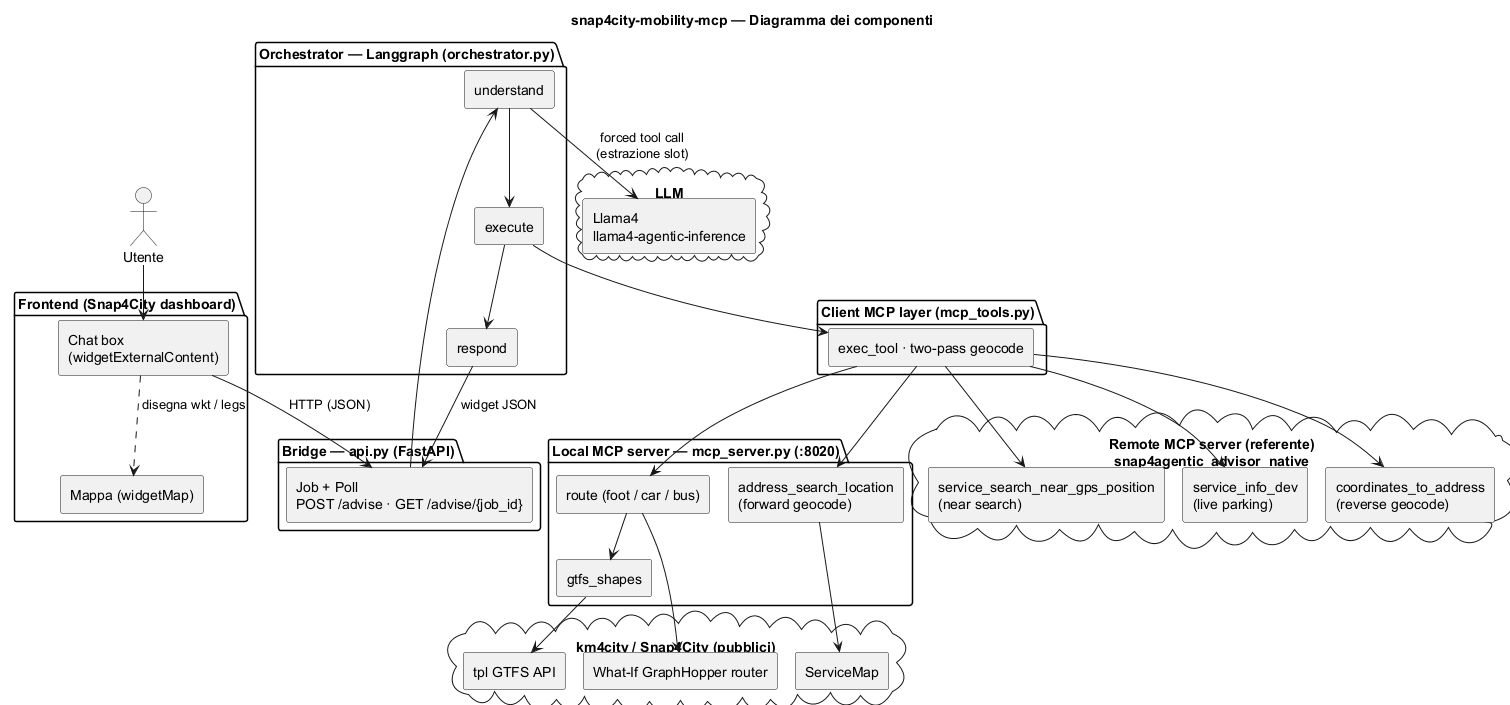
\includegraphics[width=\textwidth]{component.png}
  \caption{Diagramma dei componenti: front-end, bridge, orchestratore, i due server MCP
           e i servizi esterni.}
  \label{fig:component}
\end{figure}

La ripartizione degli strumenti fra i due server MCP non \`e arbitraria.
La geocodifica diretta e il routing sono serviti dal \textbf{server mobility} perch\'e i
corrispondenti tool nativi non erano utilizzabili:

\begin{itemize}
  \item il tool remoto \texttt{address\_search\_location} restituisce, per una via
        fiorentina, zero risultati toscani (i primi sono ad Anversa e in Grecia) e non
        ordina per punteggio di rilevanza; nessun parametro dello schema permette di
        correggerlo. Il server mobility interroga direttamente la ServiceMap pubblica,
        che sulla stessa interrogazione restituisce il risultato corretto in prima
        posizione;
  \item il tool remoto \texttt{routing} non ha mai restituito trasporto pubblico reale
        e richiedeva una lunga catena di tentativi per gestire risposte vuote
        transitorie. \`E stato sostituito dal router What-If.
\end{itemize}

Restano remoti tre tool che funzionano correttamente: geocodifica inversa
(\texttt{coordinates\_to\_address}), ricerca per prossimit\`a
(\texttt{service\_search\_near\_gps\_position}) e disponibilit\`a parcheggi
(\texttt{service\_info\_dev}).

\section{Il flusso di un turno}

La Figura~\ref{fig:graphflow} descrive la logica interna del grafo.

\begin{figure}[htbp]
  \centering
  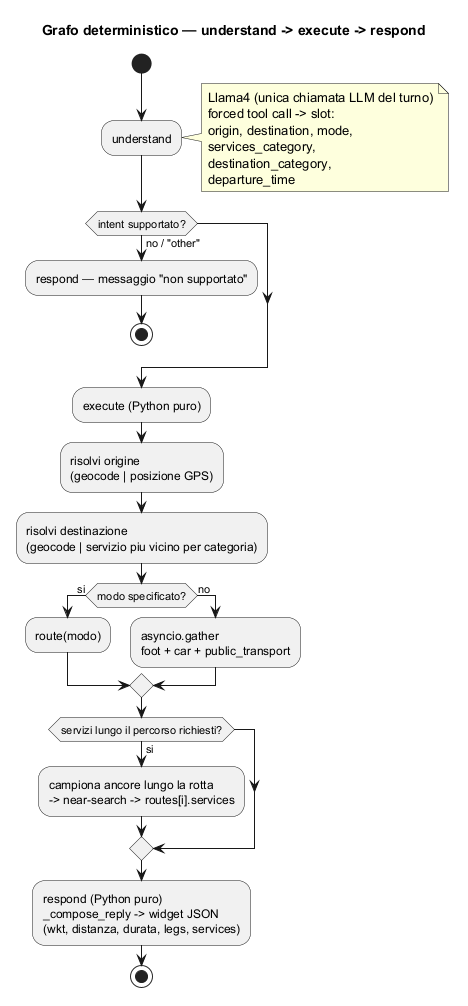
\includegraphics[width=0.72\textwidth,height=0.82\textheight,keepaspectratio]{graph-flow.png}
  \caption{Grafo deterministico: il modello interviene solo nel nodo
           \texttt{understand}.}
  \label{fig:graphflow}
\end{figure}

% =====================================================================
\chapter{Implementazione}

\section{Estrazione dei parametri}

Il nodo \texttt{understand} invia la domanda dell'utente, insieme agli ultimi turni di
conversazione, con una chiamata a strumento forzata. Lo schema estrae:
intento, testo dell'origine, testo della destinazione, modo di trasporto, categoria di
destinazione (per richieste generiche come \emph{``la farmacia pi\`u vicina''}),
categoria dei servizi da mostrare lungo il percorso e orario di partenza. Fra i valori
dell'intento rientra anche la \textbf{ricerca di soli servizi vicini} (\emph{pins-only}),
che riusa la categoria di destinazione come categoria da cercare e il testo dell'origine
come centro, senza aggiungere nuovi parametri allo schema.

La cronologia inviata al modello \`e limitata agli ultimi otto messaggi: il contesto
per un \emph{follow-up} sta negli ultimi turni, mentre una cronologia illimitata
amplifica la latenza e il rischio di errori del gateway.

\section{Risoluzione degli estremi del percorso}

\`E la parte con pi\`u casistica, perch\'e l'indice geografico non offre alcun
parametro di vincolo territoriale. La strategia \`e a scalini:

\begin{enumerate}
  \item \textbf{Doppia passata}: prima si cercano solo indirizzi
        (\texttt{excludePOI=true}), le cui coordinate cadono sul grafo stradale; si
        ricade sui punti di interesse solo se la prima passata non produce risultati
        nella citt\`a indicata. Senza questo accorgimento
        \emph{``Piazza del Duomo''} restituisce prima un'azienda omonima.
  \item \textbf{Citt\`a nominata}: se l'utente nomina una citt\`a, i candidati vengono
        ristretti a quella.
  \item \textbf{Ancoraggio}: altrimenti si sceglie il candidato pi\`u vicino a un punto
        di riferimento --- la destinazione si ancora all'origine gi\`a risolta,
        l'origine alla posizione GPS. Senza l'ancoraggio, \emph{``via Pisana 166''}
        partendo da Firenze veniva risolta a Lucca, con un percorso di 65~km
        formalmente corretto ma sbagliato nei fatti.
  \item \textbf{Numero civico}: se il testo contiene un numero civico si privilegia la
        corrispondenza esatta sul campo \texttt{civic}, poi le etichette di forma
        stradale, e solo da ultimo la vicinanza all'ancora. Le interrogazioni senza
        numero civico non sono toccate da questo scalino.
  \item \textbf{Reinterrogazione con la citt\`a dell'ancora}: l'indice ordina per sola
        rilevanza testuale e tronca i risultati, quindi la via omonima della citt\`a
        dell'utente pu\`o non comparire affatto fra i candidati. Se l'utente non ha
        nominato una citt\`a, la ricerca viene ripetuta aggiungendo il nome della
        citt\`a dedotta. Un controllo sui \emph{token} significativi evita che un punto
        di riferimento di un'altra citt\`a (\emph{``Piazza dei Miracoli''}) venga
        attirato erroneamente.
\end{enumerate}

Se l'origine manca del tutto, si usa la posizione GPS del browser, geocodificata a
ritroso una sola volta per poter dire \emph{``dalla tua posizione''}; in assenza di GPS
il sistema chiede il punto di partenza invece di indovinare.

\section{Calcolo dei percorsi}

Quando l'utente non indica un modo, i tre profili vengono calcolati
\textbf{concorrentemente} con un unico \texttt{asyncio.gather} piatto, e il turno
risponde una sola volta quando tutti sono pronti: il tempo totale \`e quello del pi\`u
lento, non la somma. Se il modo \`e indicato esplicitamente si calcola solo quello, in
modo che chi chiede un percorso a piedi non paghi la latenza del trasporto pubblico.

I tre risultati non hanno per\`o la stessa struttura. A piedi e in auto sono itinerari
\textbf{monomodali}: un unico mezzo copre l'intero tragitto, dall'origine alla
destinazione. Quello con il trasporto pubblico \`e invece \textbf{multimodale}, perch\'e
combina un tratto pedonale fino alla fermata di salita, una o pi\`u tratte a bordo
dell'autobus e un tratto pedonale finale. Per questo il back-end lo restituisce
suddiviso in tratte (\texttt{legs}), ciascuna con la propria geometria e il proprio
mezzo, mentre per un itinerario monomodale \`e sufficiente un'unica geometria: \`e la
suddivisione che permette al front-end di disegnare con colori distinti la parte a piedi
e quella in autobus, e di collocare i segnaposto alle fermate di salita e di discesa.

L'eventuale orario di partenza viene passato \emph{solo} al profilo di trasporto
pubblico, l'unico con un modello temporale (gli orari GTFS); il fuso orario viene
fissato esplicitamente a \texttt{Europe/Rome}, perch\'e il servlet interpreta le date
prive di offset nel proprio fuso e il processo sul JupyterHub lavora in UTC.

Un itinerario di trasporto pubblico che il router restituisce interamente pedonale non
\`e un errore: su tragitti brevi camminare domina qualunque attesa. In quel caso il
percorso perde la propria natura multimodale e viene ri-etichettato come pedonale,
presentato onestamente come tale.

\section{La geometria reale delle tratte in autobus}

Per una tratta percorsa in autobus il router restituisce \textbf{un vertice per fermata}:
la geometria reale del percorso non \`e presente nella sua risposta, quindi la linea
disegnata taglia gli isolati in linea retta.

Il modulo \texttt{gtfs\_shapes.py} la recupera a runtime dall'API pubblica \emph{tpl} di
km4city: individua la variante di linea che corrisponde alla tratta e ne ritaglia il tratto
compreso fra la fermata di salita e quella di discesa. Quando nessuna variante corrisponde,
la tratta conserva la geometria originale: la funzionalit\`a degrada, non fallisce.

\section{Il front-end}

La chat box \`e un \texttt{widgetExternalContent} incollato nella dashboard, che
disegna i percorsi su un \texttt{widgetMap} adiacente. Il widget dispone di un ramo
\emph{manual} che collega semplicemente i punti forniti: usandolo, la mappa
\textbf{non interroga alcun router} e la linea compare insieme al testo della risposta.
Per l'itinerario multimodale il back-end invia la suddivisione in tratte a piedi e in
autobus, che vengono disegnate con colori distinti e con i segnaposto alle fermate di
salita e discesa.

Quando un turno restituisce pi\`u percorsi, una barra di \emph{chip} permette di
selezionarne uno: la selezione \`e \textbf{puramente locale} --- ridisegna la mappa,
mostra il dettaglio gi\`a pre-calcolato dal back-end e commuta i segnaposto --- perch\'e
un nuovo turno costerebbe di nuovo la latenza dell'autobus. Nella cronologia conversazionale
viene riscritta solo una riga di eco della scelta, sufficiente a mantenere il contesto
per le domande successive senza gonfiare i prompt seguenti.

% =====================================================================
\chapter{Distribuzione e integrazione}

Il sistema gira sulla \textbf{JupyterHub di Snap4City}, unico ambiente da cui sono
raggiungibili sia i due server MCP (ospitati sul server Snap4City, rete interna) sia
l'endpoint del modello. Come mostra la Figura~\ref{fig:deployment}, la JupyterHub esegue
\textbf{un solo processo}, il bridge FastAPI sulla porta 8010; il server mobility \`e
ospitato sul server Snap4City e non va pi\`u avviato a mano. Il browser raggiunge il
bridge \emph{same-origin} attraverso \texttt{jupyter-server-proxy}.

\begin{figure}[htbp]
  \centering
  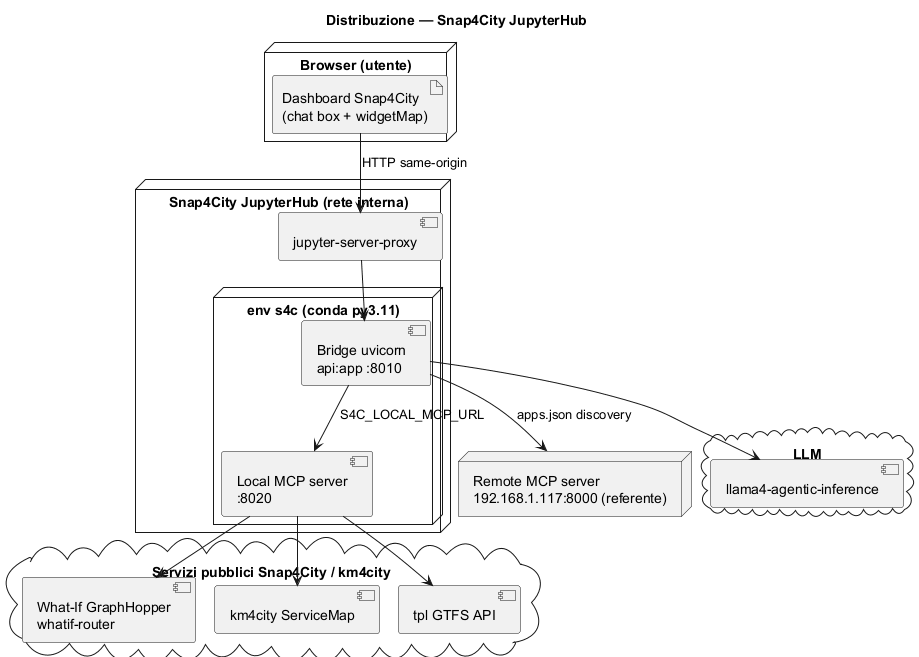
\includegraphics[width=0.95\textwidth]{deployment.png}
  \caption{Distribuzione: un solo processo (il bridge) nell'ambiente JupyterHub, i due
           server MCP sul server Snap4City, la dashboard nel browser, i servizi esterni.}
  \label{fig:deployment}
\end{figure}

% =====================================================================
\chapter{Casistica applicativa}
\label{cap:casistica}

Questo capitolo raccoglie gli scenari d'uso supportati dall'advisor, catturati
sulla dashboard reale. Per ciascuno si riportano: la \emph{situazione}, la
\emph{riproduzione} (il tipo di richiesta e le eventuali precondizioni, come il
GPS del browser), il \emph{riferimento} all'output completo allegato in \texttt{examples/} e la relativa
schermata. Gli indirizzi di prova
usano il numero civico completo (cos\`i la risoluzione civica \`e esercitata in ogni
scenario di percorso) e localit\`a toscane, dove i dati km4city sono validi. Le schermate
sono indicizzate anche in \texttt{screenshots/README.md}.

% ---------------------------------------------------------------------
\section{Percorsi punto-punto}

\subsection{S01 --- Tre modi (nessun modo indicato)}
\textbf{Situazione.} Senza indicare il modo, l'advisor calcola e disegna insieme i tre
itinerari (a piedi, in auto, trasporto pubblico) e offre le chip di selezione.
\textbf{Riproduzione.} L'utente chiede il percorso tra due indirizzi civici, senza indicare il modo.
\textbf{Output completo:} \exfile{S01-tre-modi}.
\begin{figure}[htbp]
  \centering
  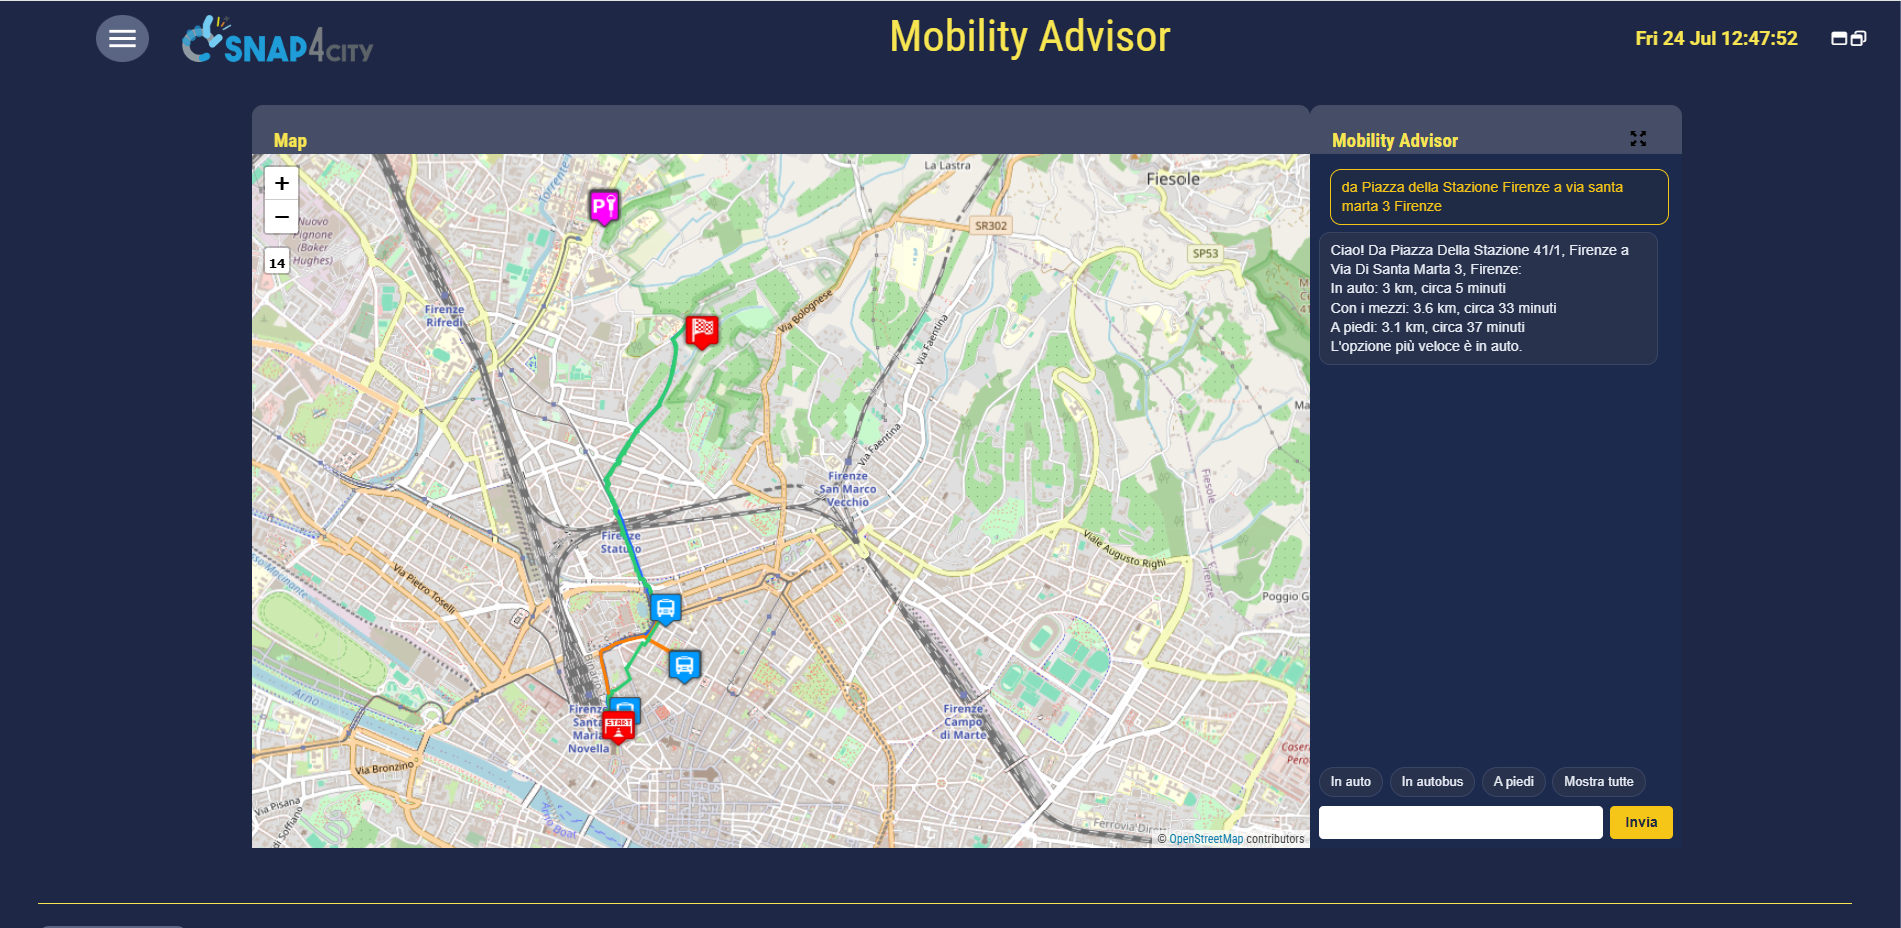
\includegraphics[width=\textwidth]{S01-tre-modi.jpg}
  \caption{Turno a tre modi: le tre rotte disegnate insieme, il testo di confronto e il
           dock delle chip.}
  \label{fig:S01}
\end{figure}

\subsection{S02 --- Chip ``A piedi''}
\textbf{Situazione.} Dallo stato a tre modi, la selezione di una chip ridisegna localmente
la sola rotta scelta e apre la bolla di dettaglio, senza un nuovo turno verso il bridge.
\textbf{Riproduzione.} Dopo S01, clic sulla chip \emph{A piedi}.
\textbf{Output:} vista lato client del payload di \exfile{S01-tre-modi}.
\begin{figure}[htbp]
  \centering
  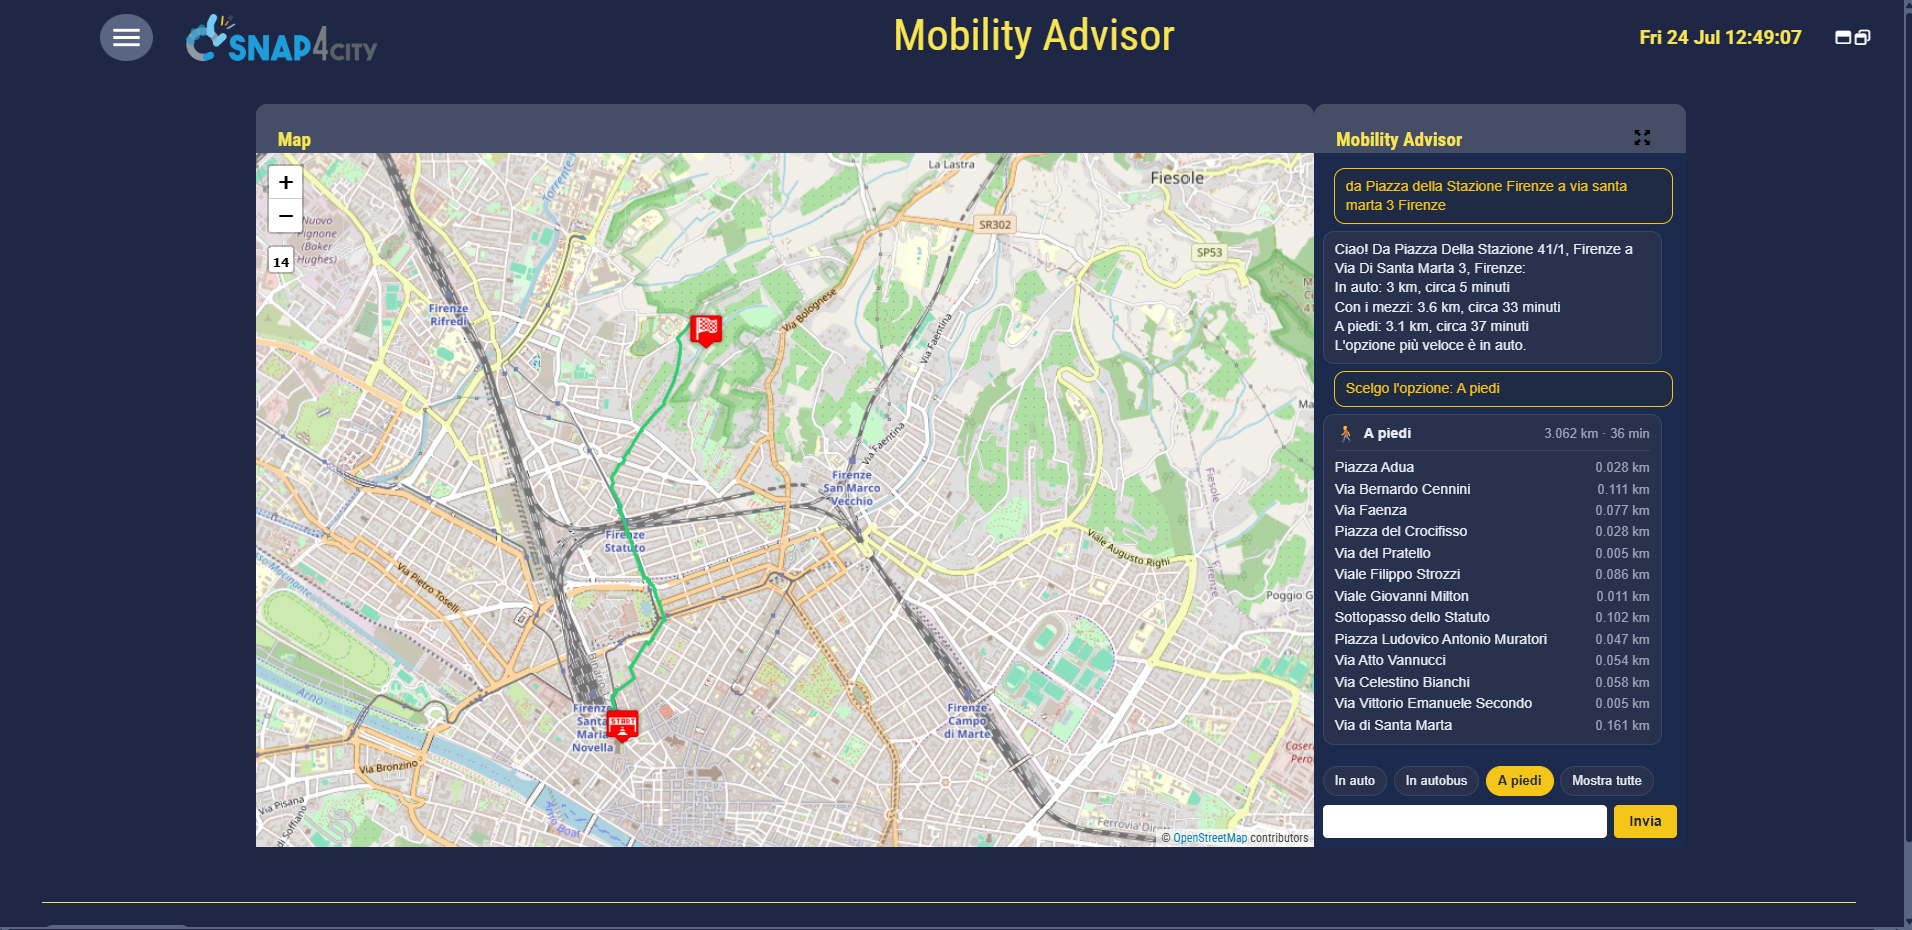
\includegraphics[width=\textwidth]{S02-tre-modi-piedi.jpg}
  \caption{Selezione della chip pedonale: la sola rotta a piedi e la bolla di dettaglio.}
  \label{fig:S02}
\end{figure}

\subsection{S03 --- Chip ``In auto''}
\textbf{Situazione.} La chip auto mostra la sola rotta in auto, il dettaglio e i pin dei
parcheggi vicini alla destinazione.
\textbf{Riproduzione.} Dopo S01, clic sulla chip \emph{In auto}.
\textbf{Output:} vista lato client del payload di \exfile{S01-tre-modi}.
\begin{figure}[htbp]
  \centering
  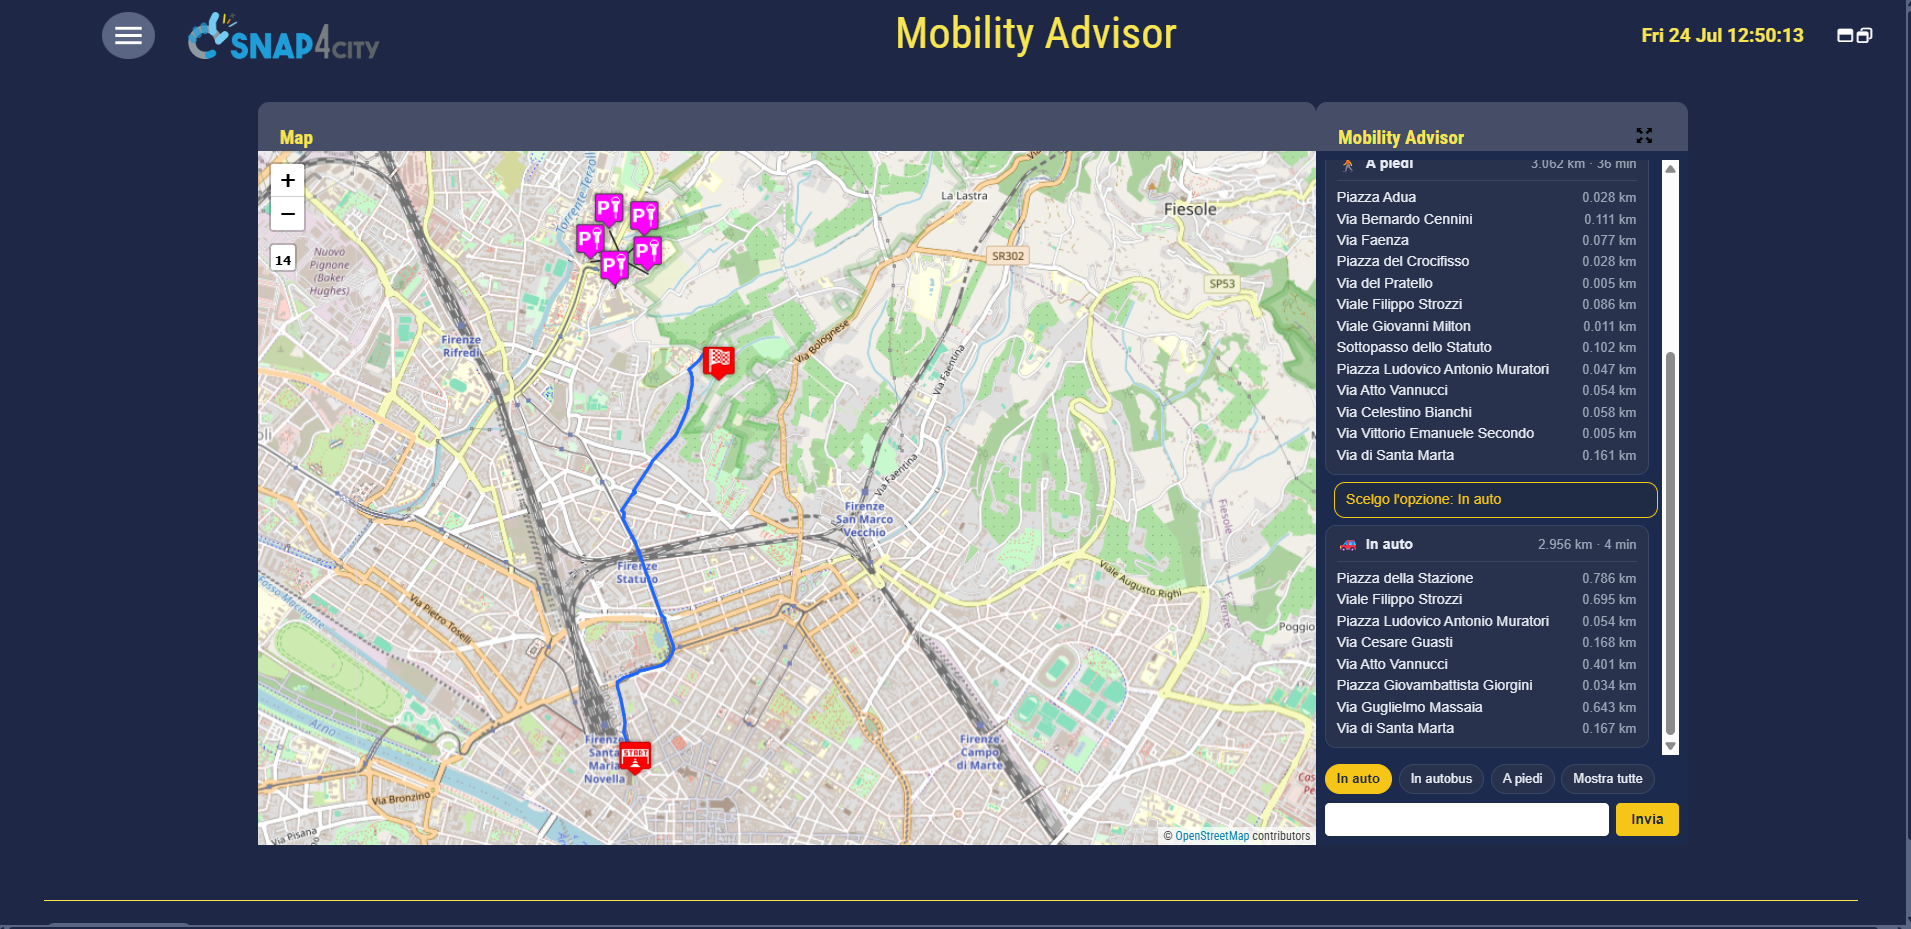
\includegraphics[width=\textwidth]{S03-tre-modi-auto.jpg}
  \caption{Chip in auto: rotta, dettaglio e pin dei parcheggi.}
  \label{fig:S03}
\end{figure}

\subsection{S04 --- Chip ``In autobus''}
\textbf{Situazione.} La chip autobus mostra il solo itinerario multimodale, con la
geometria separata per tratta (a piedi + bus) e i pin delle fermate.
\textbf{Riproduzione.} Dopo S01, clic sulla chip \emph{In autobus}.
\textbf{Output:} vista lato client del payload di \exfile{S01-tre-modi}.
\begin{figure}[htbp]
  \centering
  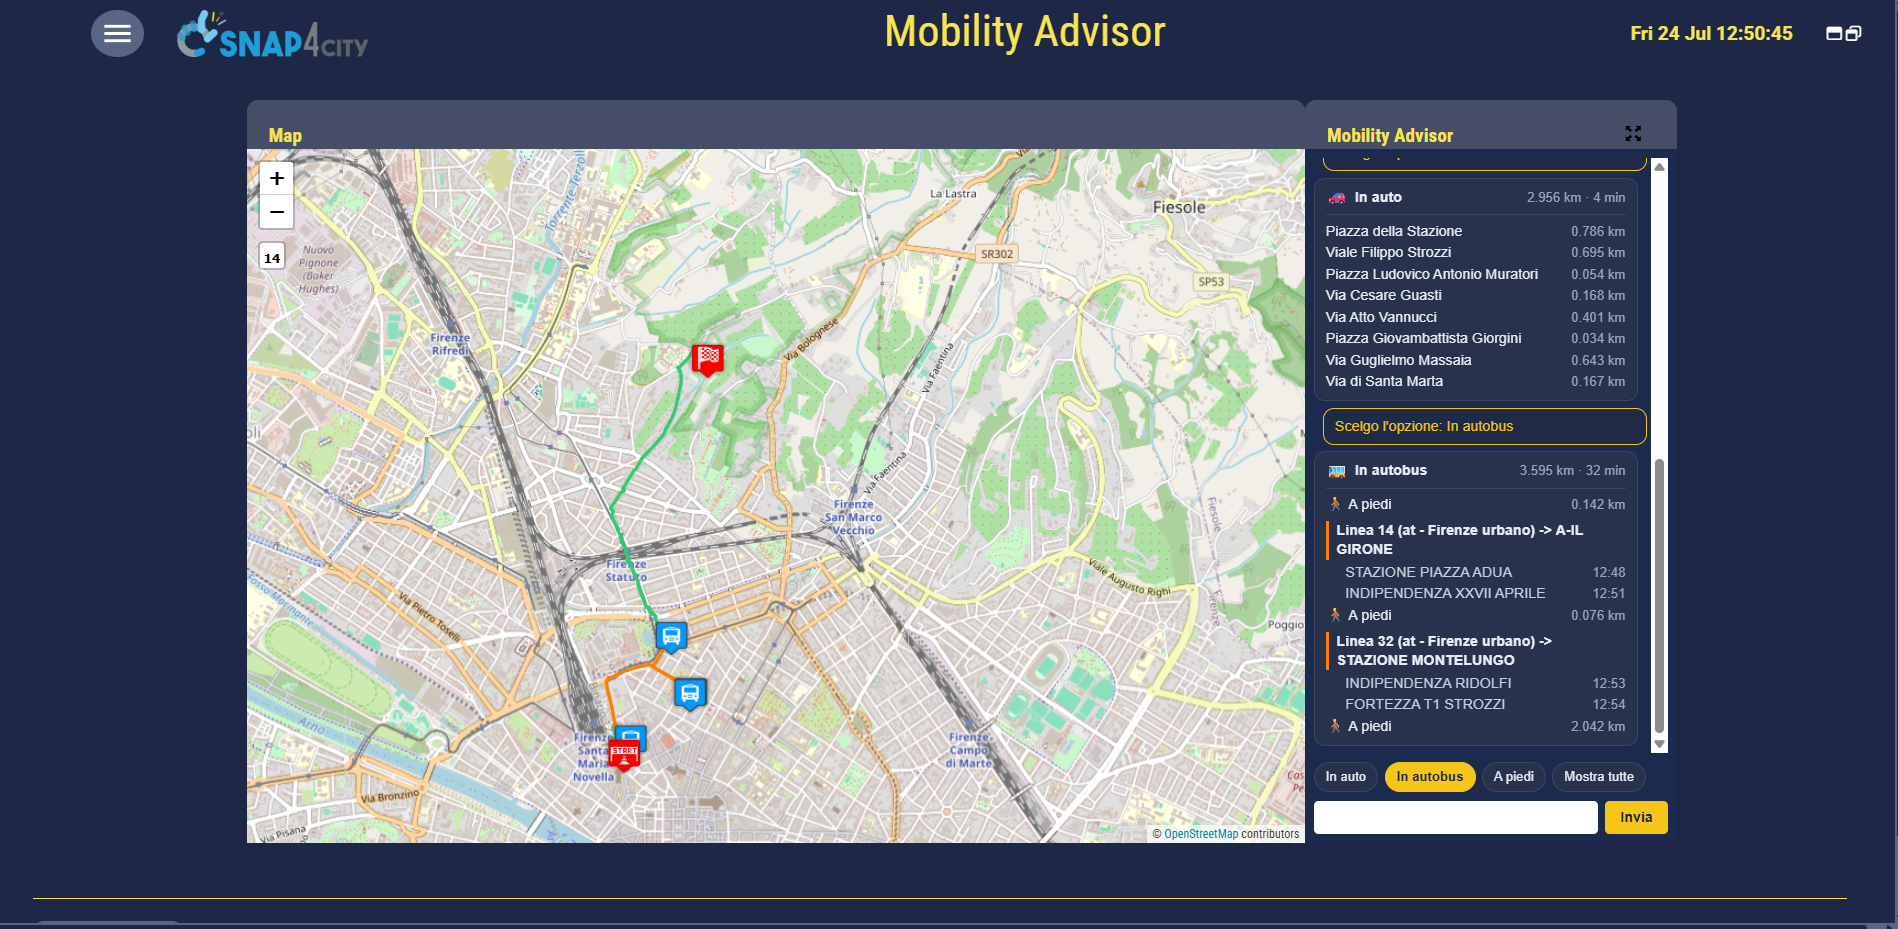
\includegraphics[width=\textwidth]{S04-tre-modi-autobus.jpg}
  \caption{Chip in autobus: itinerario per-tratta e pin delle fermate.}
  \label{fig:S04}
\end{figure}

\subsection{S05 --- Destinazione senza citt\`a: candidato pi\`u vicino}
\textbf{Situazione.} Quando l'indirizzo di destinazione non nomina la citt\`a e lo stesso
nome di via ricorre in pi\`u comuni toscani, viene scelto il candidato pi\`u vicino
all'ancora (la posizione GPS per l'origine, l'origine gi\`a risolta per la destinazione).
Nominando invece la citt\`a le si d\`a la priorit\`a (caso complementare di S10).
\textbf{Riproduzione.} Con il GPS attivo, l'utente indica come destinazione una via il cui
nome ricorre in pi\`u comuni toscani, senza nominare la citt\`a: viene risolta quella pi\`u
vicina alla posizione.
\textbf{Output completo:} \exfile{S05-senza-citta}.
\begin{figure}[htbp]
  \centering
  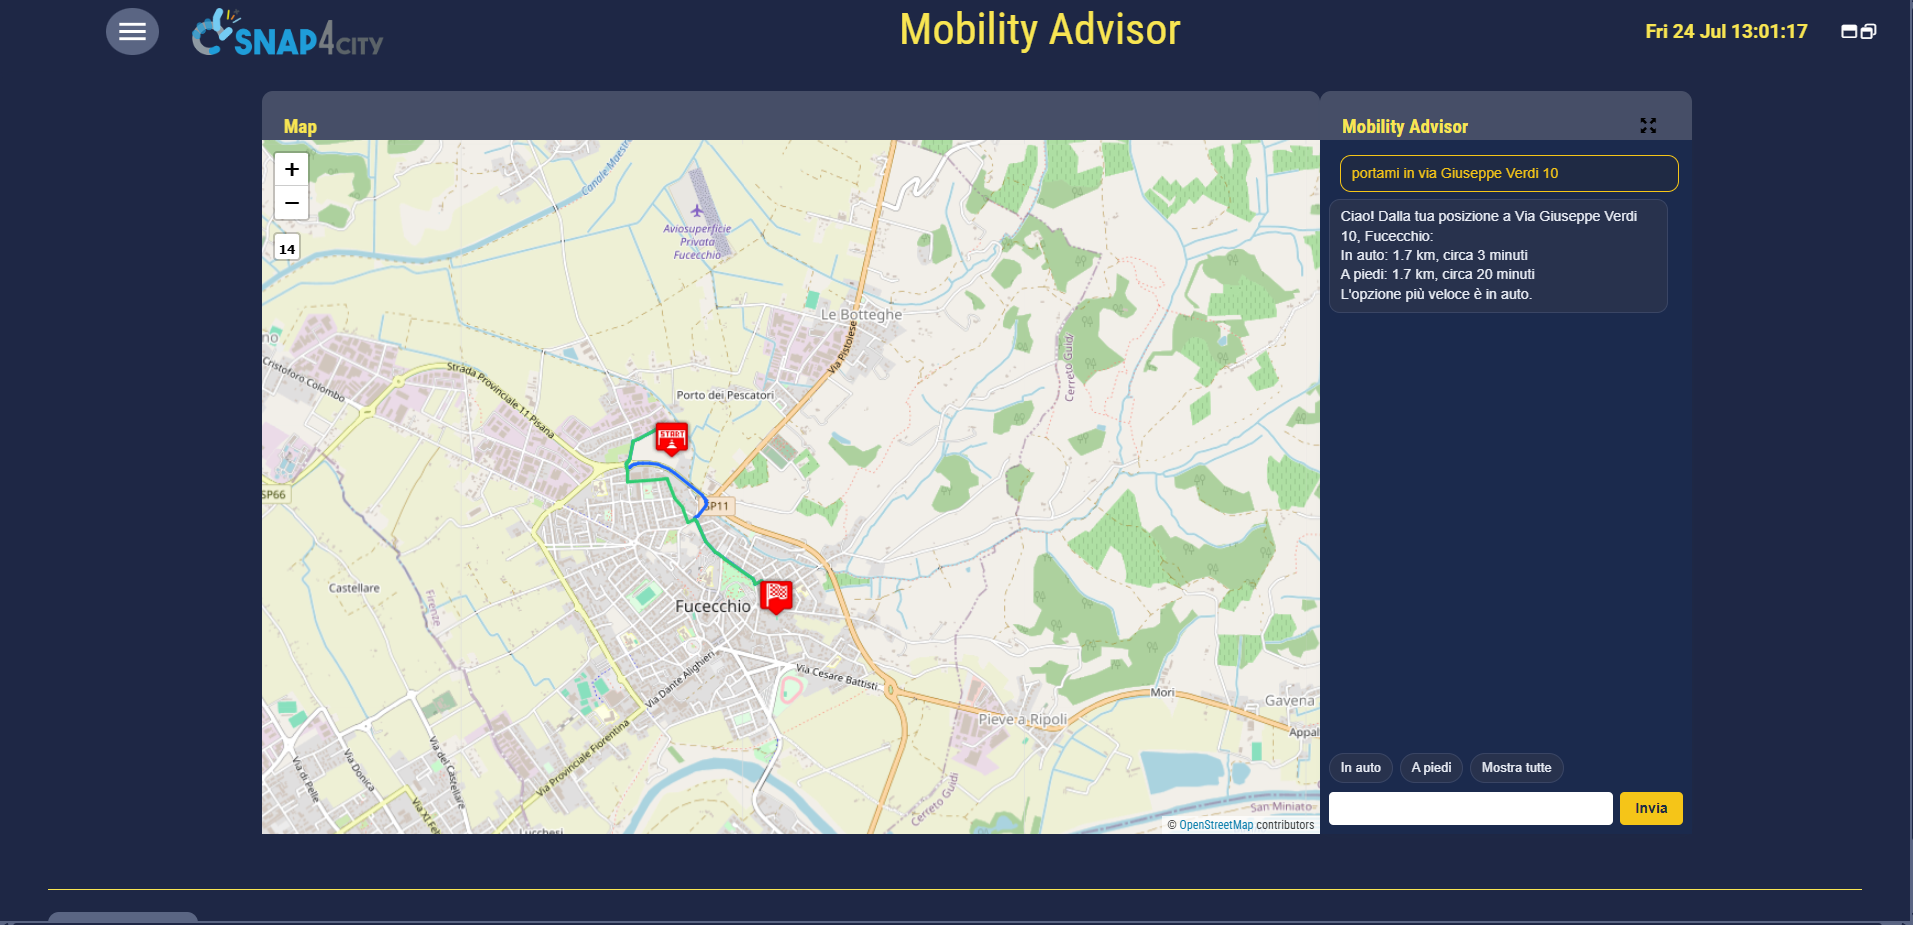
\includegraphics[width=\textwidth]{S05-senza-citta.jpg}
  \caption{Destinazione senza citt\`a risolta sul candidato pi\`u vicino alla posizione.}
  \label{fig:S05}
\end{figure}

\subsection{S06 --- Modo singolo, a piedi}
\textbf{Situazione.} Indicando esplicitamente il modo, l'advisor calcola una sola rotta
(non attende gli altri profili).
\textbf{Riproduzione.} L'utente chiede un percorso tra due indirizzi civici in modo \emph{a
piedi}.
\textbf{Output completo:} \exfile{S06-modo-singolo-piedi}.
\begin{figure}[htbp]
  \centering
  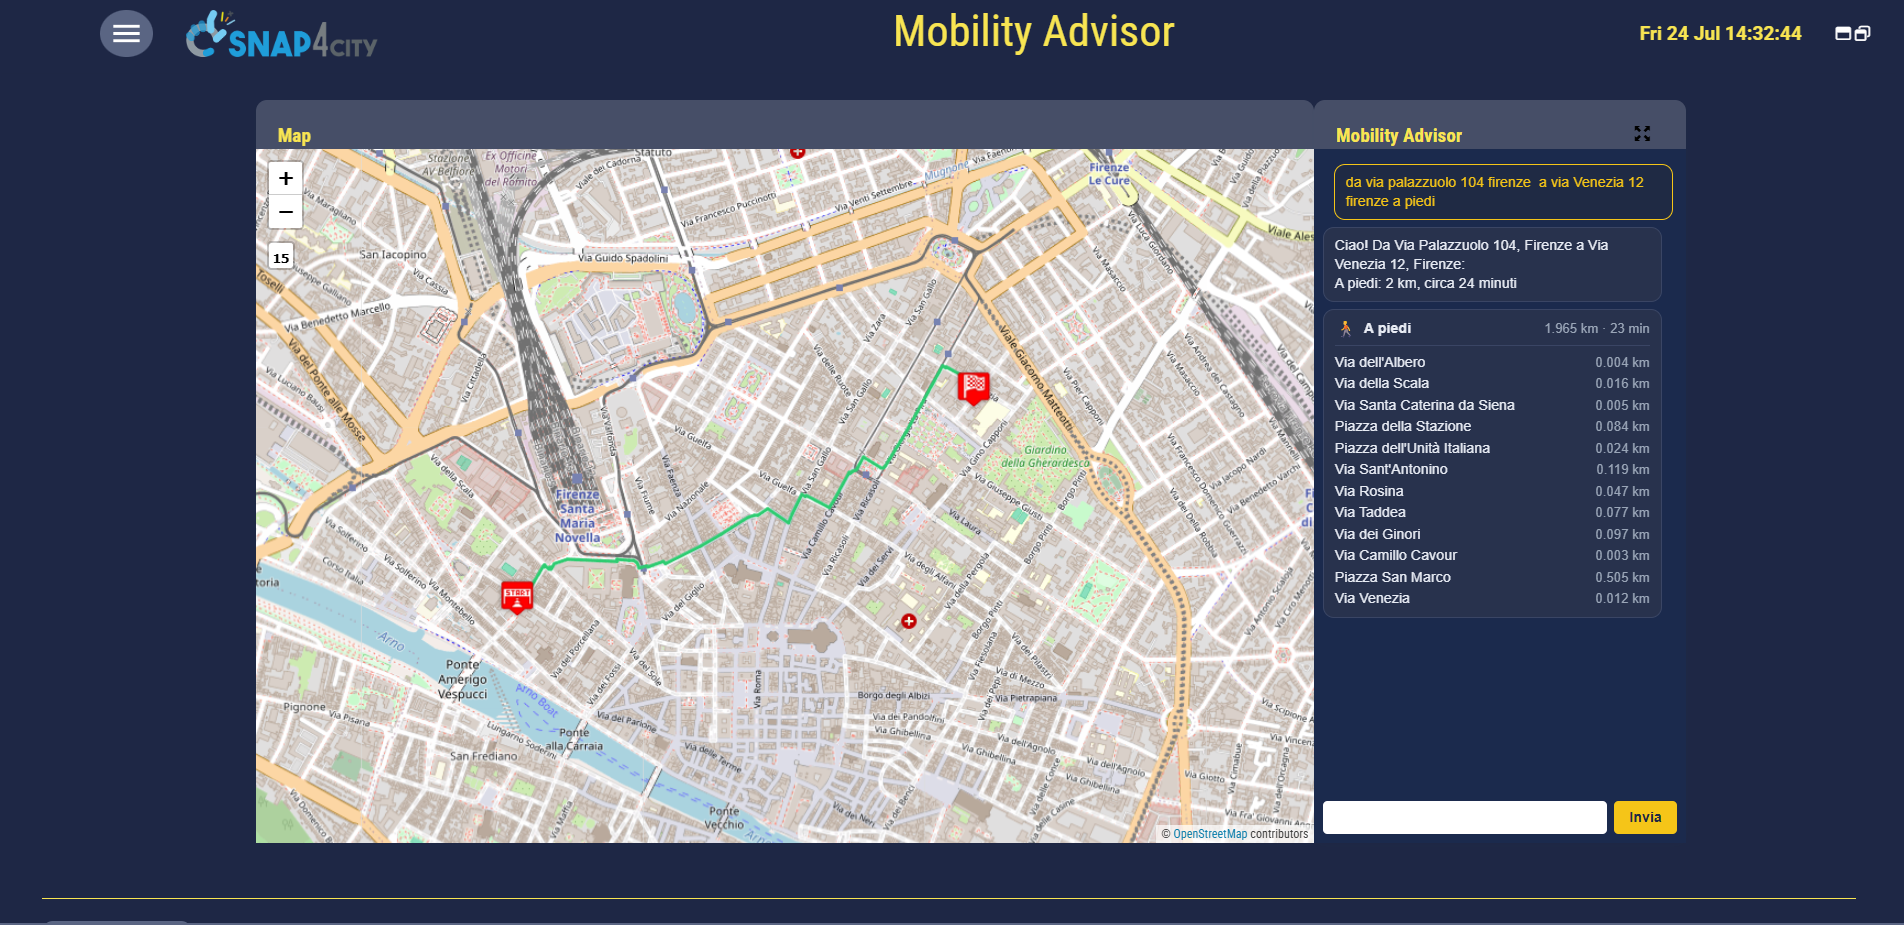
\includegraphics[width=\textwidth]{S06-modo-singolo-piedi.jpg}
  \caption{Richiesta esplicita a piedi: una sola rotta pedonale.}
  \label{fig:S06}
\end{figure}

\subsection{S07 --- Modo singolo, in auto}
\textbf{Situazione.} Come sopra, con il profilo auto.
\textbf{Riproduzione.} L'utente chiede un percorso tra due indirizzi civici in modo
\emph{auto}.
\textbf{Output completo:} \exfile{S07-modo-singolo-auto}.
\begin{figure}[htbp]
  \centering
  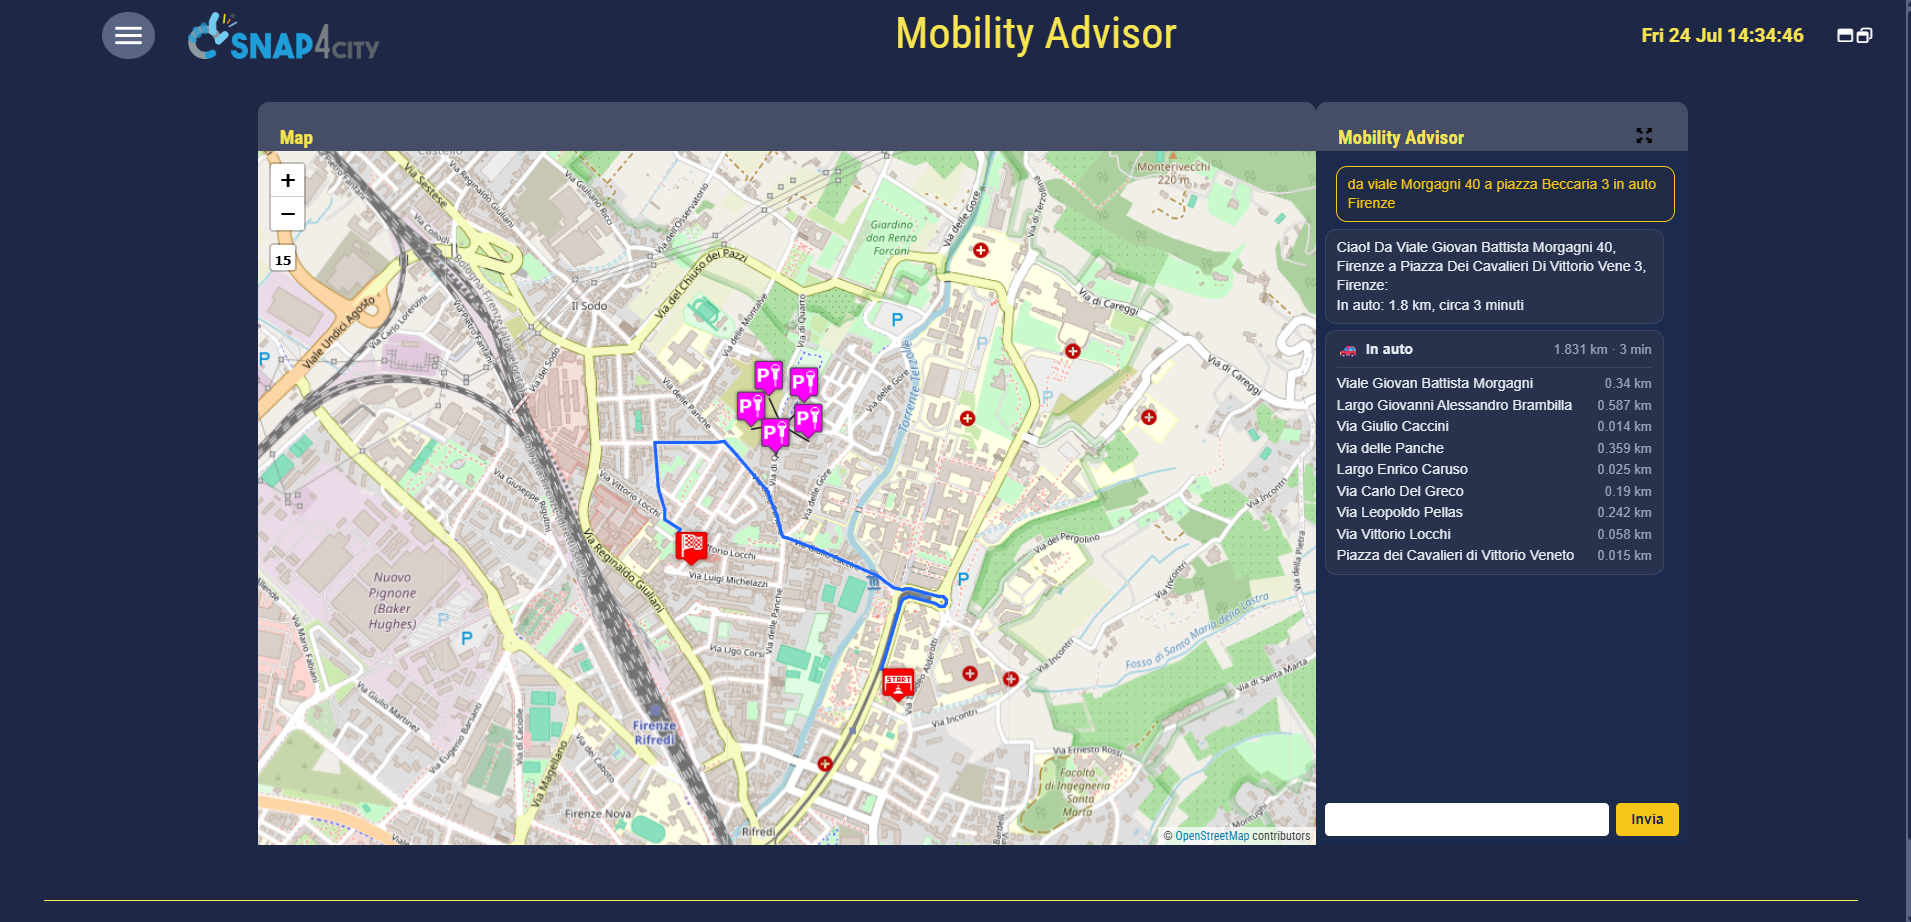
\includegraphics[width=\textwidth]{S07-modo-singolo-auto.jpg}
  \caption{Richiesta esplicita in auto: una sola rotta.}
  \label{fig:S07}
\end{figure}

\subsection{S08 --- Modo singolo, in autobus}
\textbf{Situazione.} Il solo itinerario multimodale; \`e il caso pi\`u lento (il router
ricostruisce il grafo del trasporto pubblico a ogni richiesta).
\textbf{Riproduzione.} L'utente chiede un percorso tra due indirizzi civici in modo
\emph{autobus}.
\textbf{Output completo:} \exfile{S08-modo-singolo-autobus}.
\begin{figure}[htbp]
  \centering
  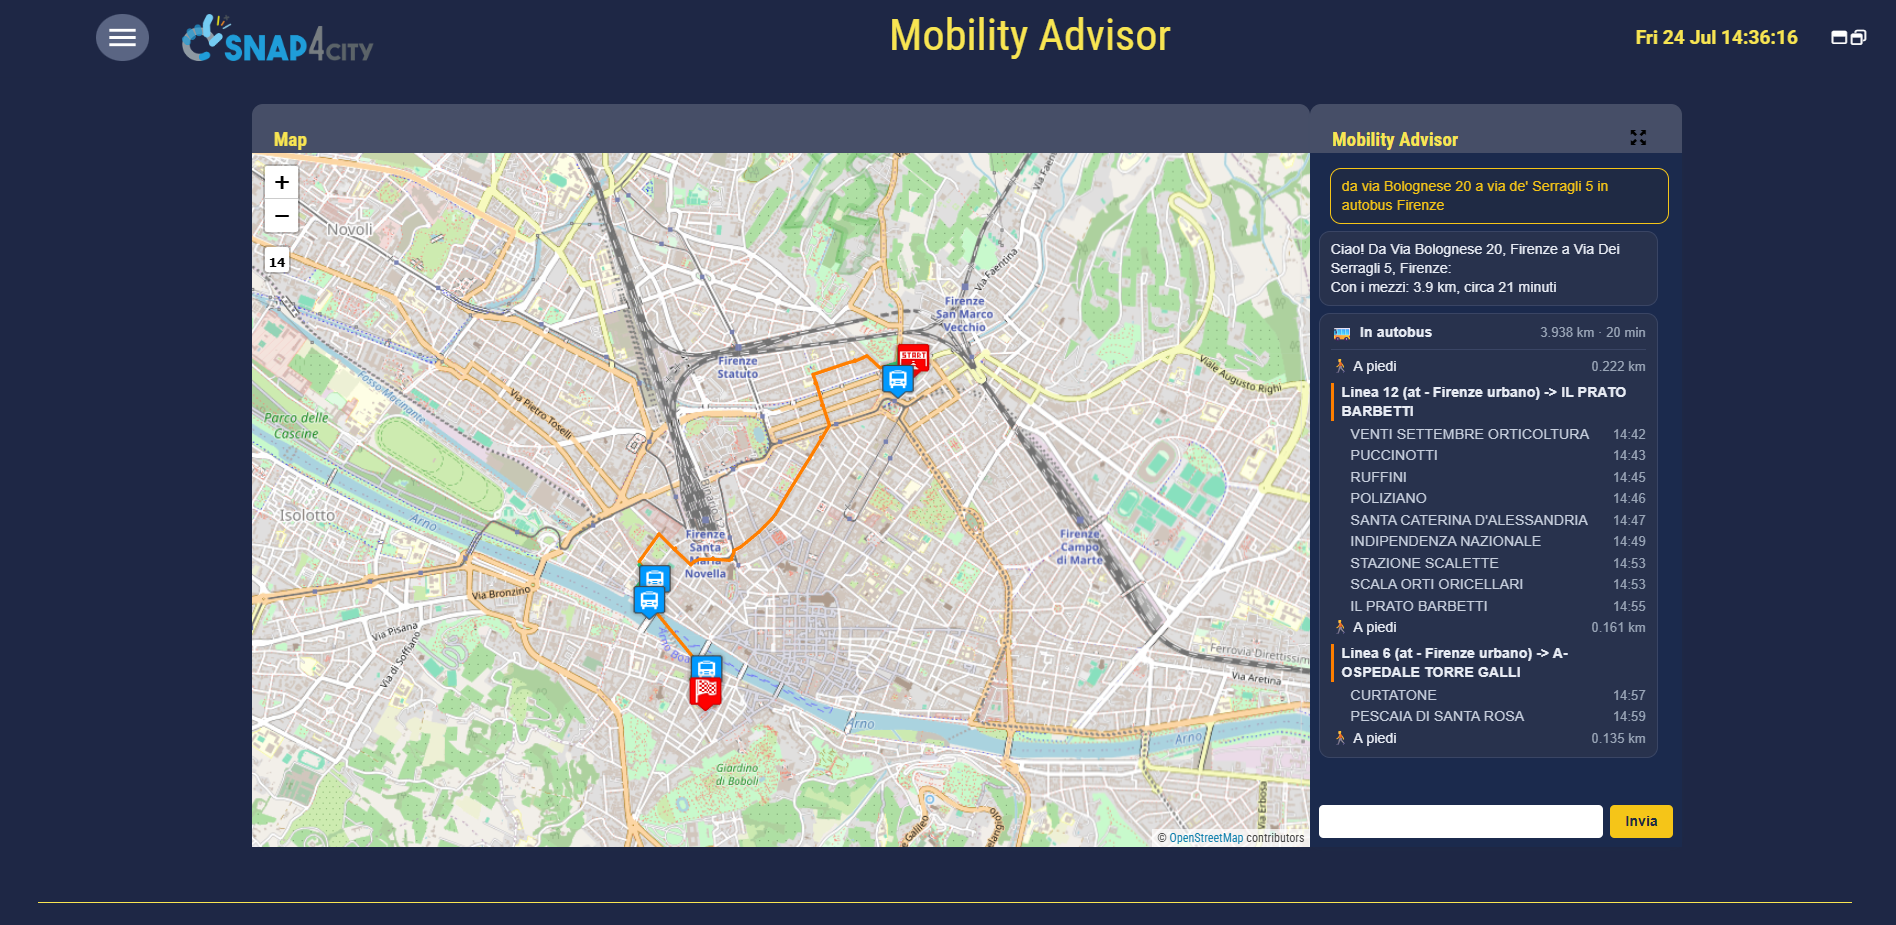
\includegraphics[width=\textwidth]{S08-modo-singolo-autobus.jpg}
  \caption{Richiesta esplicita in autobus: itinerario multimodale con fermate.}
  \label{fig:S08}
\end{figure}

% ---------------------------------------------------------------------
\section{Risoluzione degli estremi}

\subsection{S09 --- Origine dalla posizione GPS}
\textbf{Situazione.} Se l'utente non indica l'origine, viene usata la posizione GPS del
browser (etichettata tramite geocodifica inversa).
\textbf{Riproduzione.} Con il GPS attivo, l'utente indica solo la destinazione (un indirizzo
civico), senza la partenza.
\textbf{Output completo:} \exfile{S09-origine-gps}.
\begin{figure}[htbp]
  \centering
  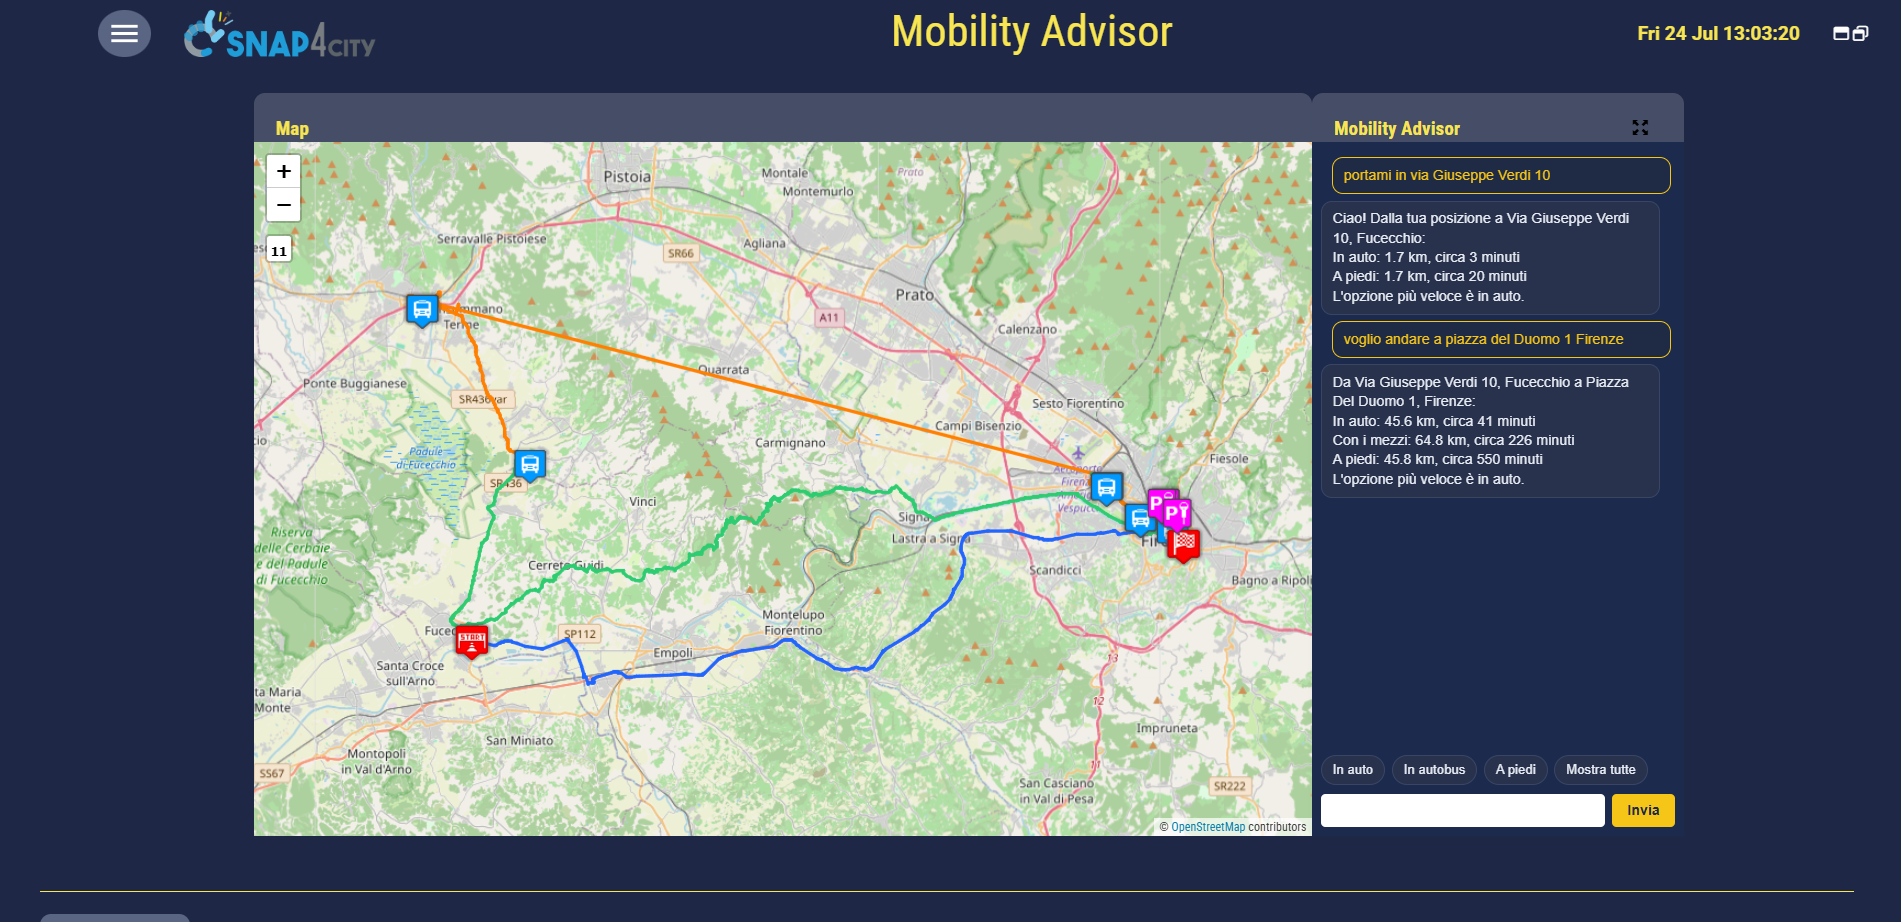
\includegraphics[width=\textwidth]{S09-origine-gps.jpg}
  \caption{Origine presa dal GPS, destinazione risolta da testo.}
  \label{fig:S09}
\end{figure}

\subsection{S10 --- Citt\`a nominata nell'indirizzo}
\textbf{Situazione.} Quando l'indirizzo nomina la citt\`a, la risoluzione le d\`a la
priorit\`a rispetto alla vicinanza all'ancora (caso complementare di S05).
\textbf{Riproduzione.} L'utente chiede un percorso tra due indirizzi indicando
esplicitamente la citt\`a di uno di essi.
\textbf{Output completo:} \exfile{S10-citta-nominata}.
\begin{figure}[htbp]
  \centering
  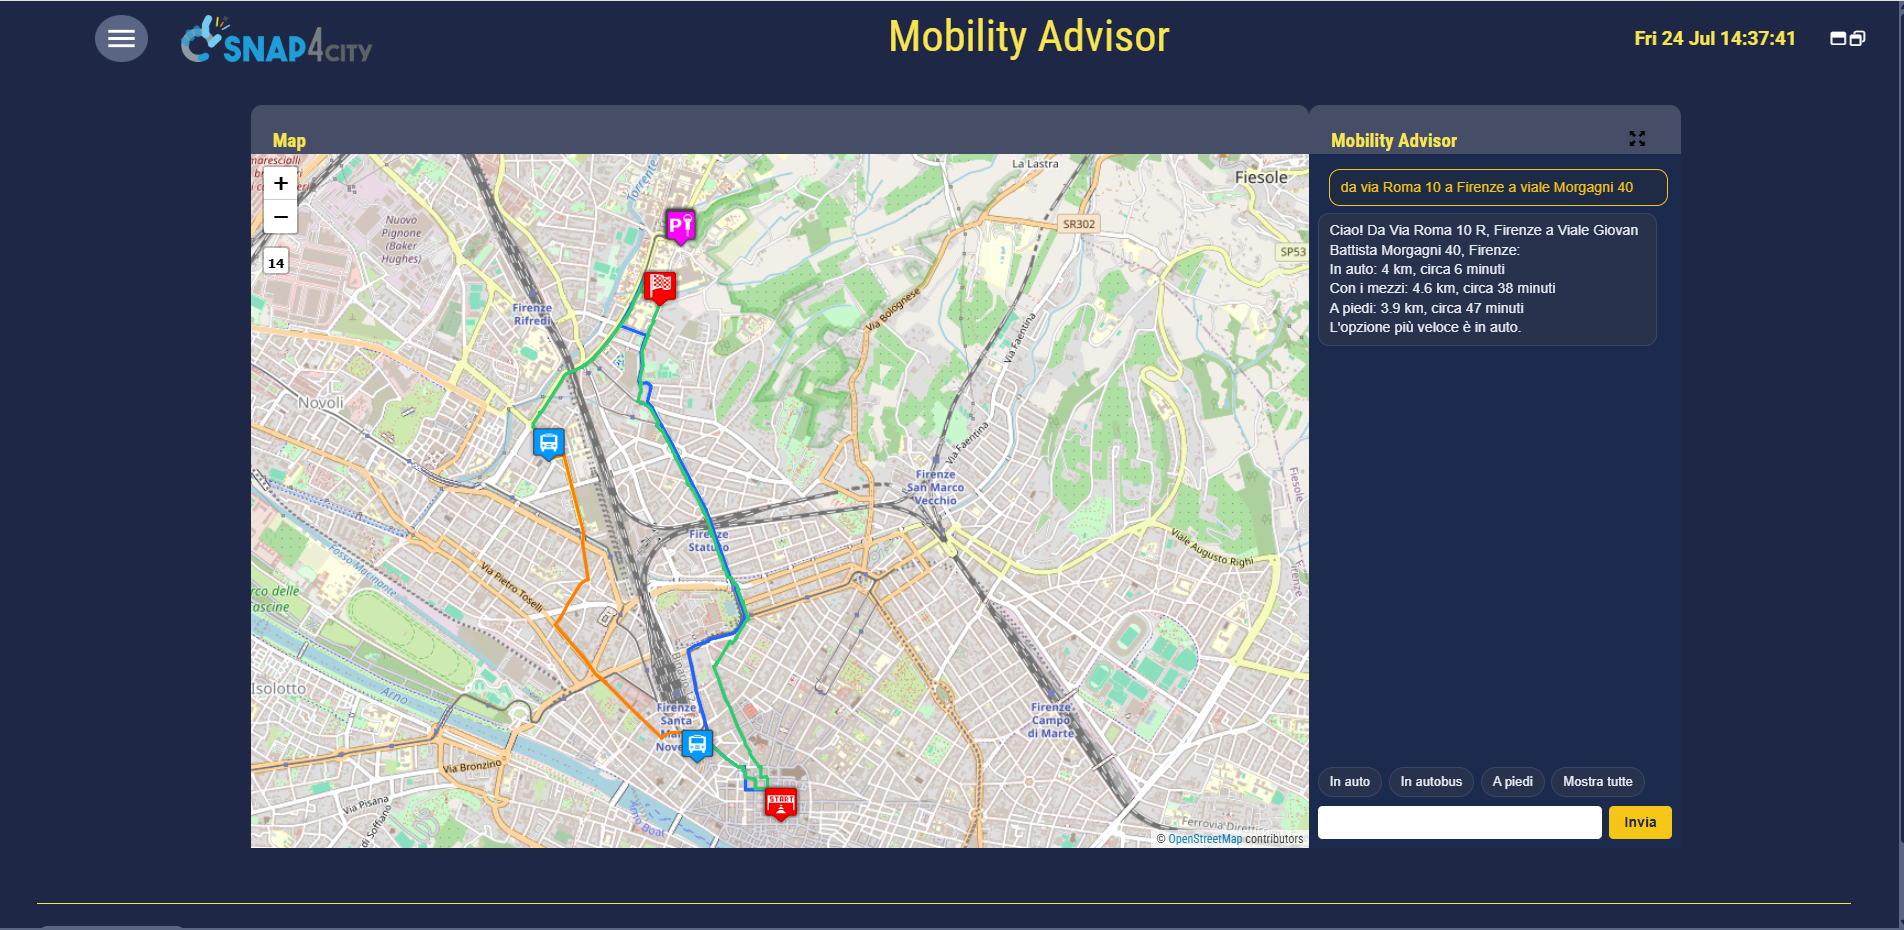
\includegraphics[width=\textwidth]{S10-citta-nominata.jpg}
  \caption{Risoluzione con priorit\`a alla citt\`a indicata.}
  \label{fig:S10}
\end{figure}

\subsection{S11 --- Follow-up multi-turno}
\textbf{Situazione.} La selezione e le risposte vengono riscritte nella cronologia, cos\`i
un turno successivo pu\`o riusare gli estremi gi\`a risolti.
\textbf{Riproduzione.} Dopo S07 (in auto), l'utente digita \emph{``e in autobus?''}.
\textbf{Output completo:} \exfile{S11-follow-up}.
\begin{figure}[htbp]
  \centering
  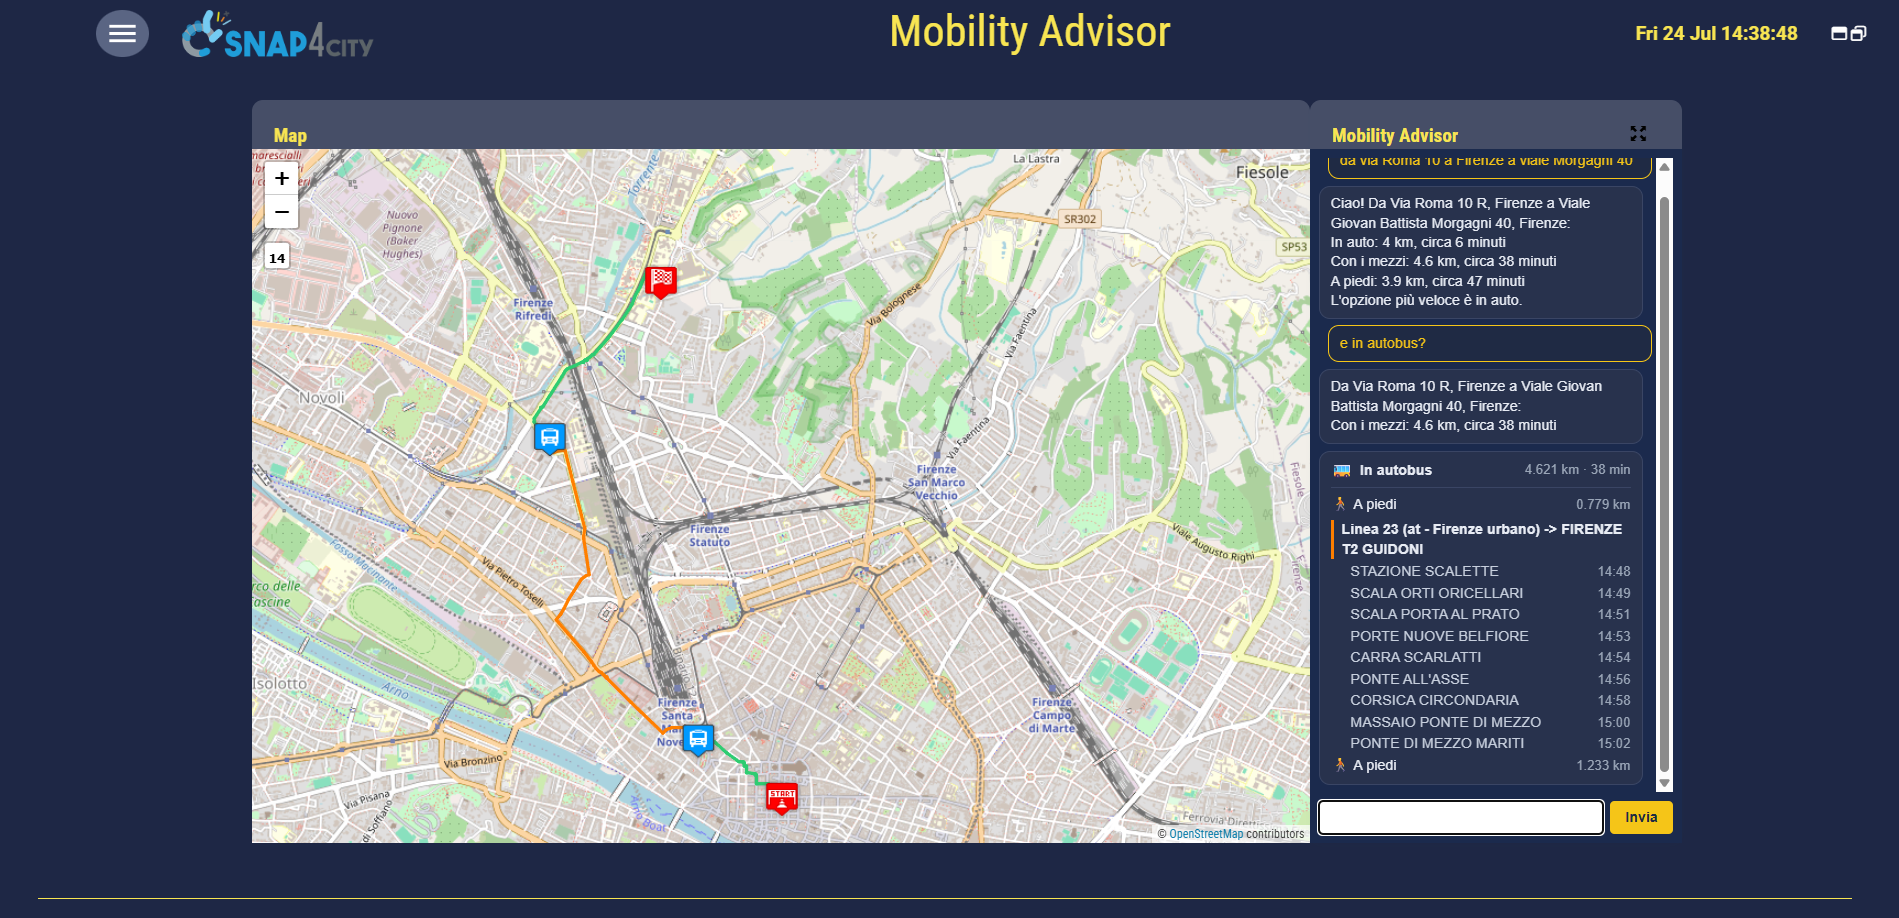
\includegraphics[width=\textwidth]{S11-follow-up.jpg}
  \caption{Il turno successivo riusa origine e destinazione dal contesto.}
  \label{fig:S11}
\end{figure}

% ---------------------------------------------------------------------
\section{Destinazione per categoria}

\subsection{S12 --- Supermercato pi\`u vicino}
\textbf{Situazione.} La destinazione \`e una categoria: l'advisor cerca il servizio pi\`u
vicino con una scala di raggio crescente (0,5 $\rightarrow$ 2 $\rightarrow$ 10 km).
\textbf{Riproduzione.} Con il GPS attivo, l'utente digita \emph{``portami al supermercato
pi\`u vicino''}.
\textbf{Output completo:} \exfile{S12-dest-categoria-supermercato}.
\begin{figure}[htbp]
  \centering
  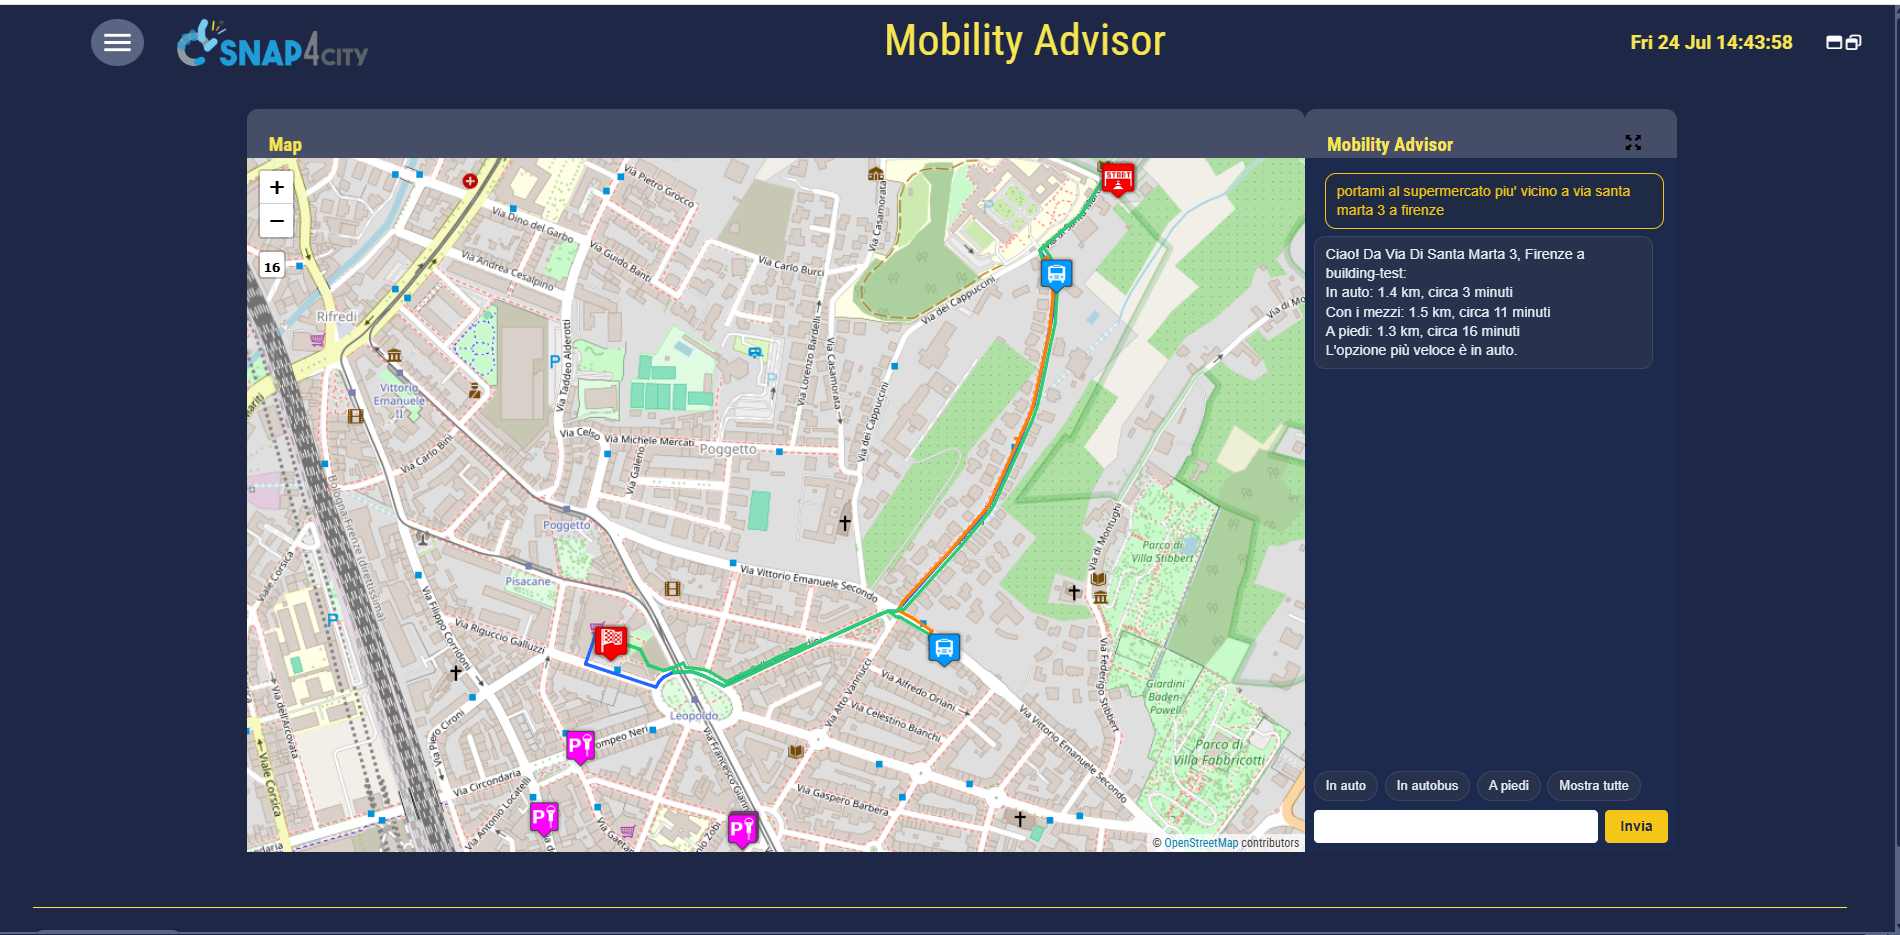
\includegraphics[width=\textwidth]{S12-dest-categoria-supermercato.jpg}
  \caption{Destinazione = supermercato pi\`u vicino alla posizione.}
  \label{fig:S12}
\end{figure}

\subsection{S13 --- Farmacia pi\`u vicina}
\textbf{Situazione.} La stessa funzione con una categoria diversa.
\textbf{Riproduzione.} Con il GPS attivo, l'utente digita \emph{``qual \`e la farmacia
pi\`u vicina?''}.
\textbf{Output completo:} \exfile{S13-dest-categoria-farmacia}.
\begin{figure}[htbp]
  \centering
  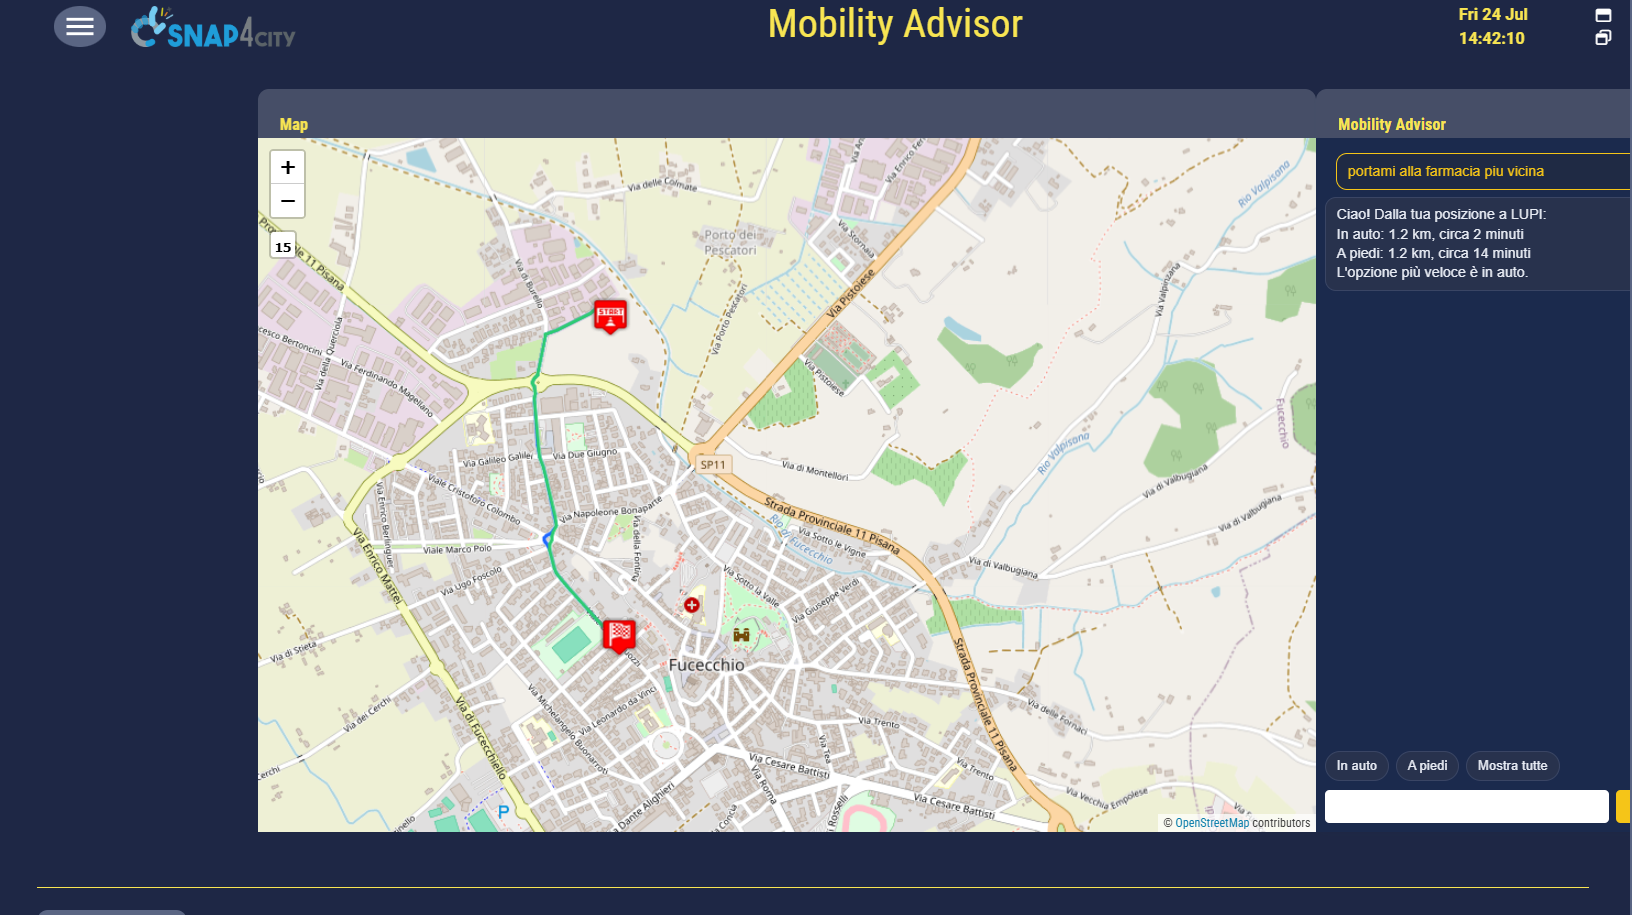
\includegraphics[width=\textwidth]{S13-dest-categoria-farmacia.jpg}
  \caption{Destinazione per categoria: farmacia pi\`u vicina.}
  \label{fig:S13}
\end{figure}

% ---------------------------------------------------------------------
\section{Servizi lungo il percorso}

\subsection{S14 --- Ristoranti lungo il percorso (in auto)}
\textbf{Situazione.} Poich\'e lo strumento remoto accetta solo un punto e un raggio, il
corridoio viene costruito lato client campionando ancore lungo la geometria del percorso
ed eseguendo una ricerca attorno a ciascuna, con deduplicazione dei risultati.
\textbf{Riproduzione.} L'utente chiede un percorso in auto tra due indirizzi e, insieme, i
ristoranti lungo il tragitto.
\textbf{Output completo:} \exfile{S14-servizi-percorso-ristoranti}.
\begin{figure}[htbp]
  \centering
  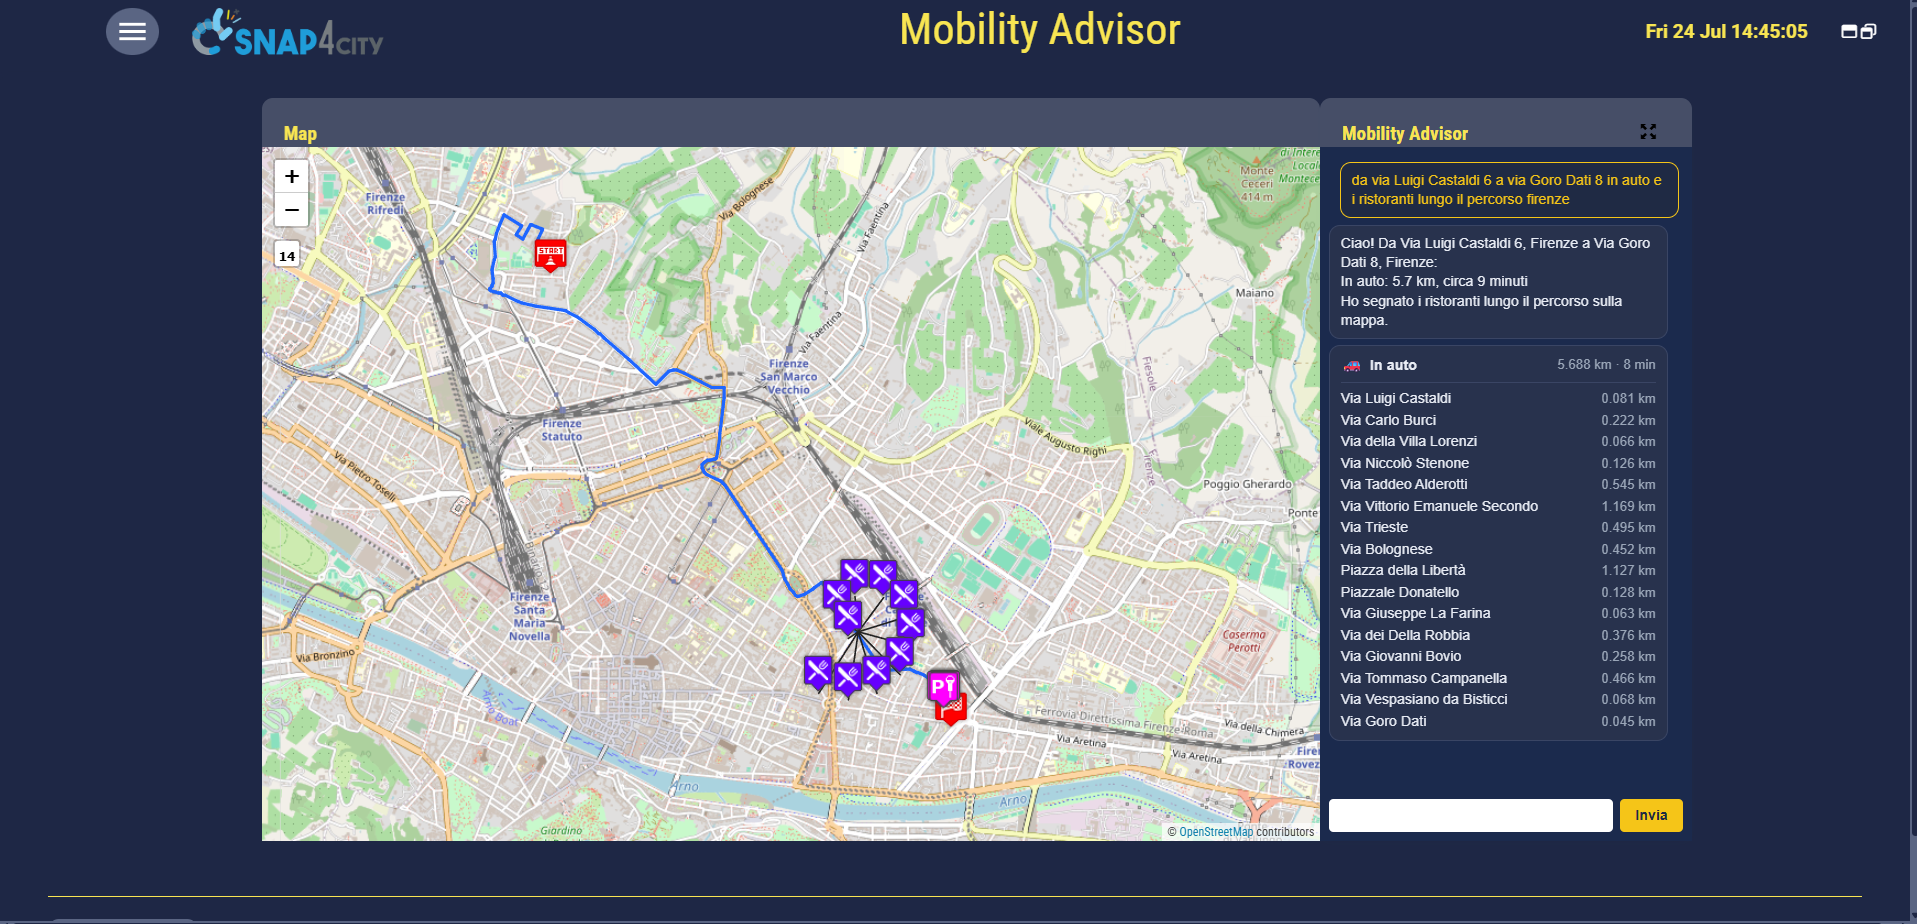
\includegraphics[width=\textwidth]{S14-servizi-percorso-ristoranti.jpg}
  \caption{Rotta in auto con i pin dei ristoranti campionati lungo il tragitto.}
  \label{fig:S14}
\end{figure}

\subsection{S15 --- Servizi lungo il percorso in autobus}
\textbf{Situazione.} In modo autobus il corridoio non segue tutta la linea: i servizi
vengono campionati solo attorno alle fermate di salita/discesa e ai tratti percorsi a
piedi.
\textbf{Riproduzione.} L'utente chiede un percorso in autobus tra due indirizzi e le farmacie
lungo il tragitto.
\textbf{Output completo:} \exfile{S15-servizi-percorso-autobus}.
\begin{figure}[htbp]
  \centering
  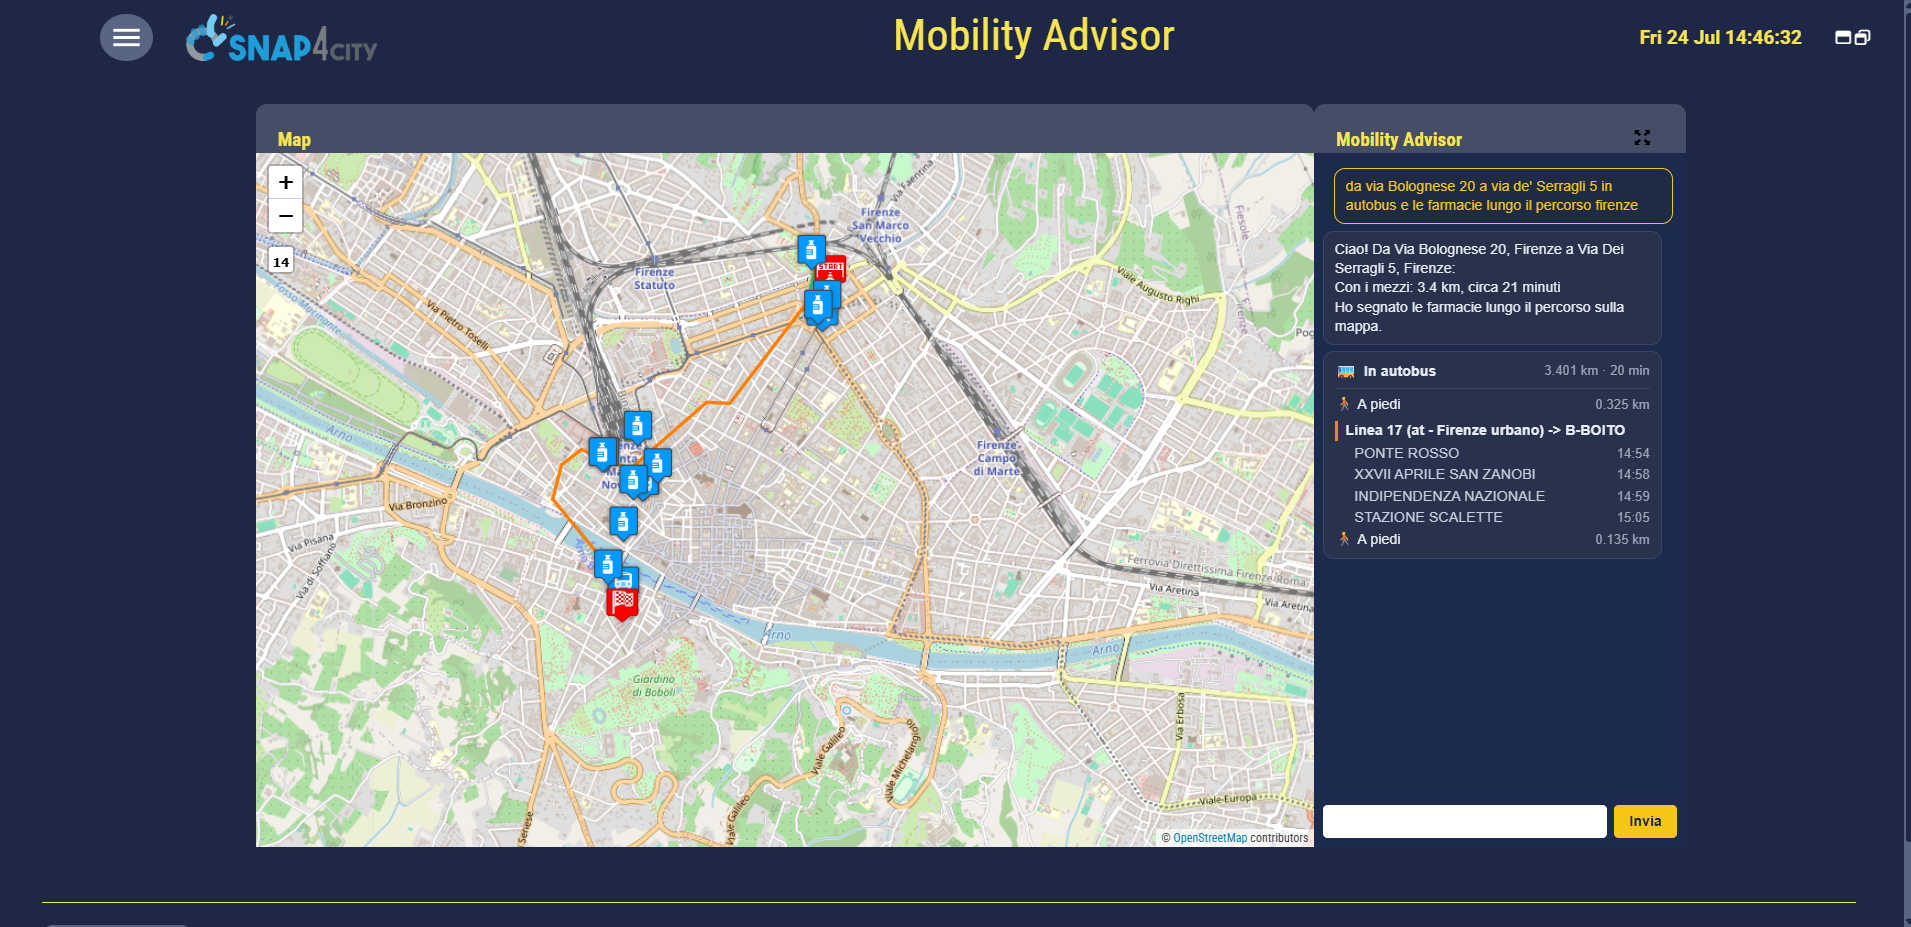
\includegraphics[width=\textwidth]{S15-servizi-percorso-autobus.jpg}
  \caption{Servizi campionati attorno a fermate e tratti a piedi dell'itinerario bus.}
  \label{fig:S15}
\end{figure}

% ---------------------------------------------------------------------
\section{Servizi vicini (senza percorso)}

\subsection{S16 --- Farmacie qui intorno (da GPS)}
\textbf{Situazione.} Una ricerca \emph{pins-only}: attorno al centro vengono cercati fino a
cinquanta servizi della categoria e restituiti come soli pin, senza tracciare alcuna
linea. Il tipo di richiesta \`e \texttt{nearby} e i servizi stanno in \texttt{data.services}.
\textbf{Riproduzione.} Con il GPS attivo, l'utente digita \emph{``mostrami le farmacie qui
intorno''}.
\textbf{Output completo:} \exfile{S16-nearby-farmacie}.
\begin{figure}[htbp]
  \centering
  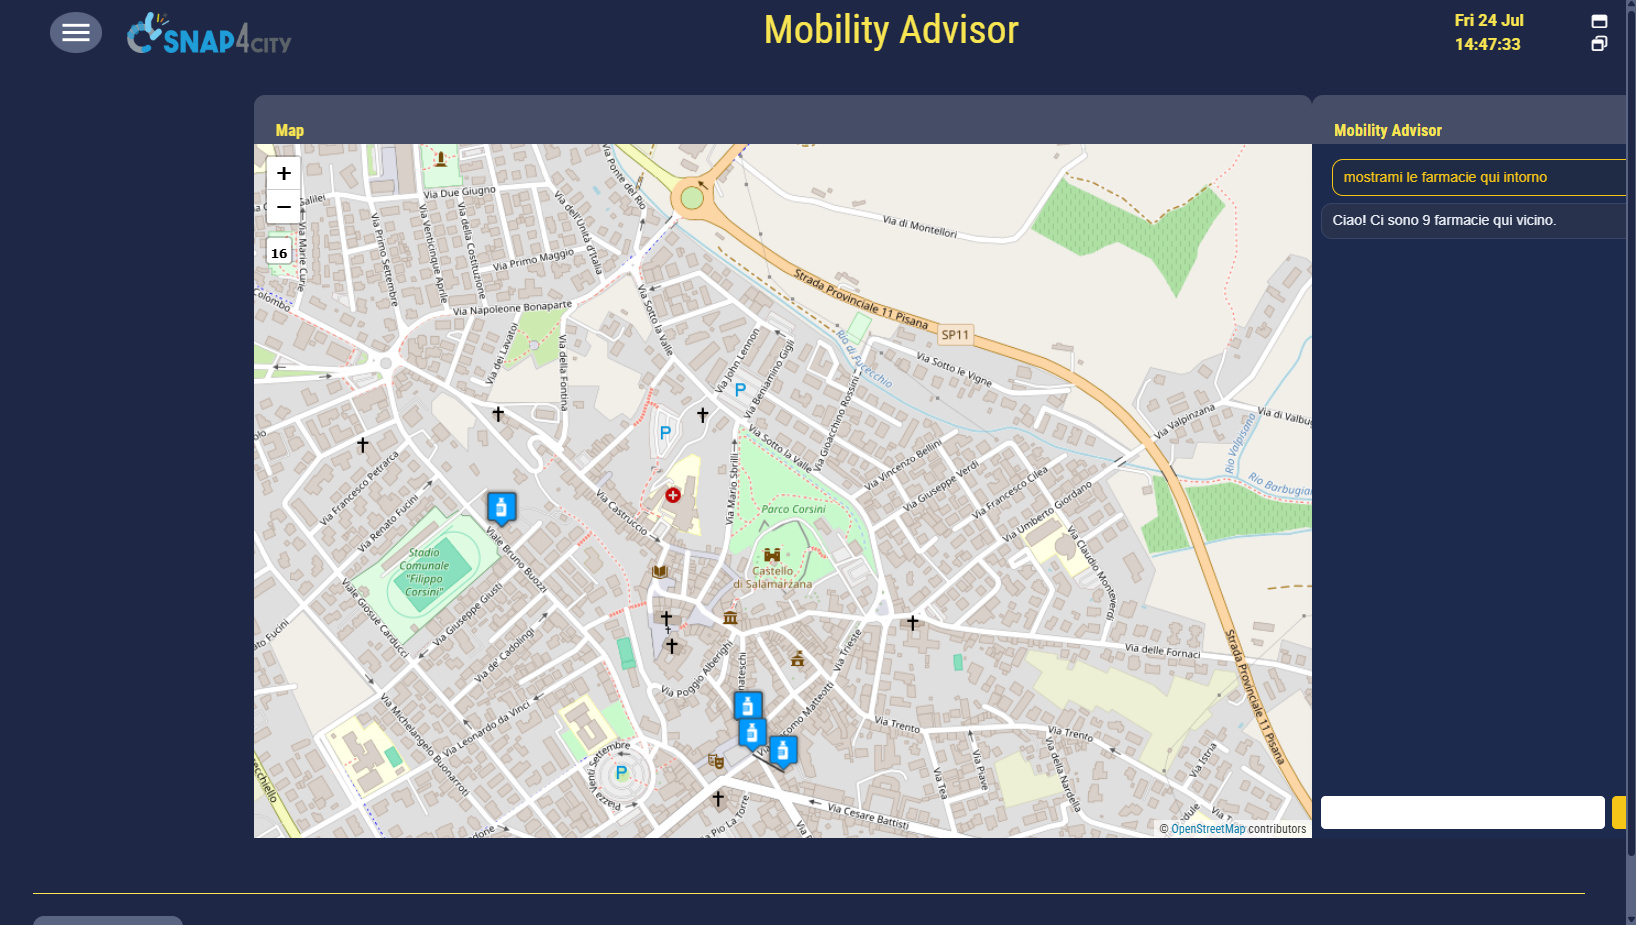
\includegraphics[width=\textwidth]{S16-nearby-farmacie.jpg}
  \caption{Solo i pin delle farmacie attorno alla posizione, senza rotta.}
  \label{fig:S16}
\end{figure}

\subsection{S17 --- Servizi vicini a un luogo nominato}
\textbf{Situazione.} Il centro della ricerca pu\`o essere un indirizzo o una citt\`a
indicati dall'utente invece della posizione GPS.
\textbf{Riproduzione.} L'utente chiede i ristoranti vicino a un luogo indicato (una piazza), non alla posizione GPS.
\textbf{Output completo:} \exfile{S17-nearby-centro-nominato}.
\begin{figure}[htbp]
  \centering
  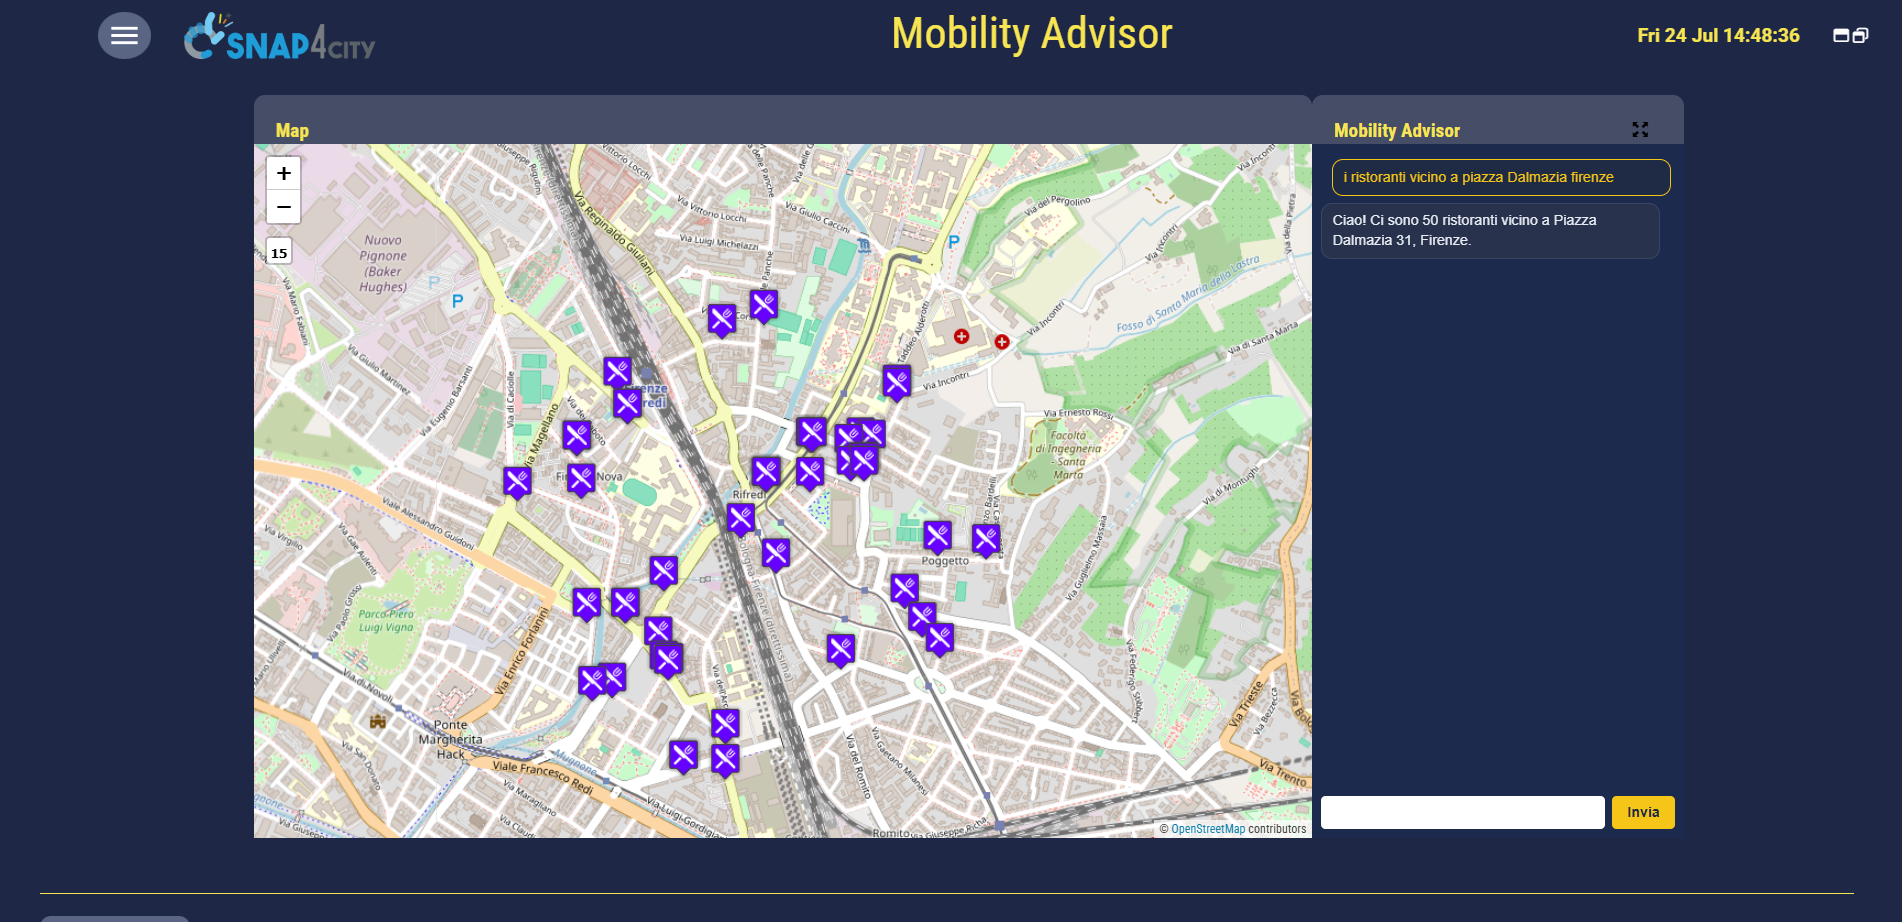
\includegraphics[width=\textwidth]{S17-nearby-centro-nominato.jpg}
  \caption{Ricerca centrata su un indirizzo indicato, non sul GPS.}
  \label{fig:S17}
\end{figure}

\subsection{S18 --- Parcheggi qui vicino}
\textbf{Situazione.} La stessa ricerca senza percorso con la categoria parcheggi.
\textbf{Riproduzione.} Con il GPS attivo, l'utente digita \emph{``dove posso parcheggiare
qui vicino?''}.
\textbf{Output completo:} \exfile{S18-nearby-parcheggi}.
\begin{figure}[htbp]
  \centering
  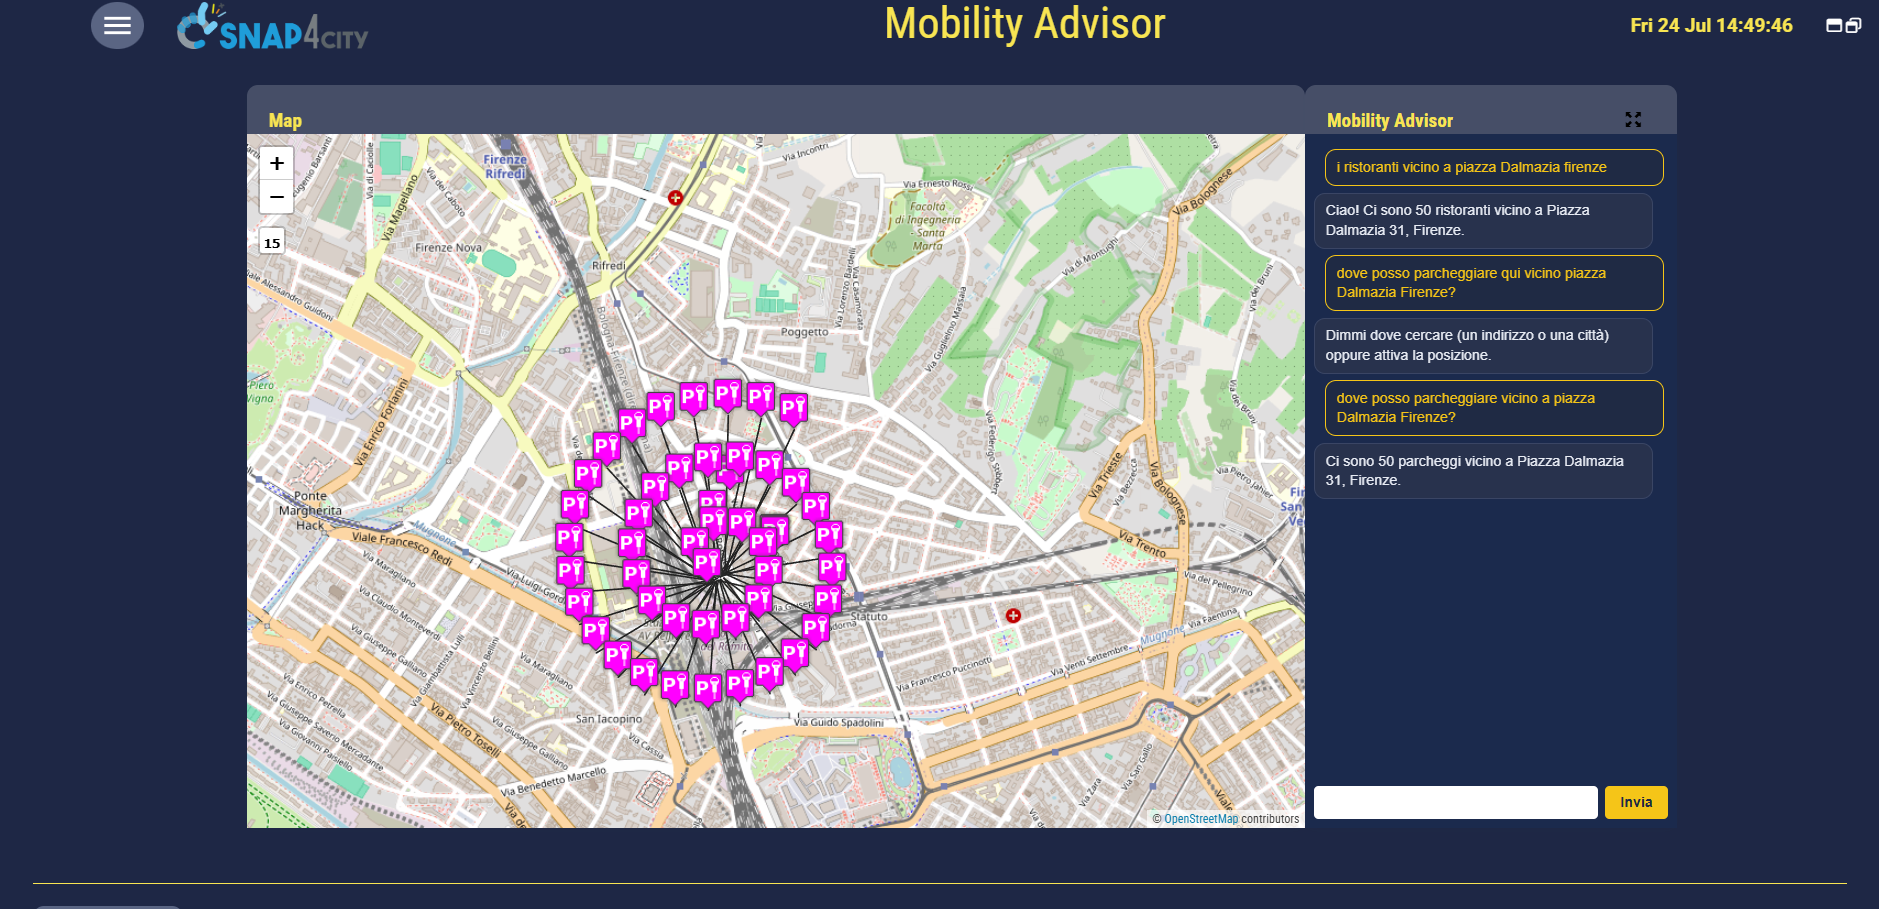
\includegraphics[width=\textwidth]{S18-nearby-parcheggi.jpg}
  \caption{Pin dei parcheggi attorno alla posizione.}
  \label{fig:S18}
\end{figure}

% ---------------------------------------------------------------------
\section{Tempo e robustezza}

\subsection{S19 --- Orario di partenza}
\textbf{Situazione.} L'orario indicato alimenta solo la pianificazione del trasporto
pubblico (i profili a piedi e auto non hanno un modello tempo-variante).
\textbf{Riproduzione.} L'utente chiede un percorso in autobus tra due indirizzi indicando
l'orario di partenza (\emph{``alle 18''}).
\textbf{Output completo:} \exfile{S19-orario-partenza}.
\begin{figure}[htbp]
  \centering
  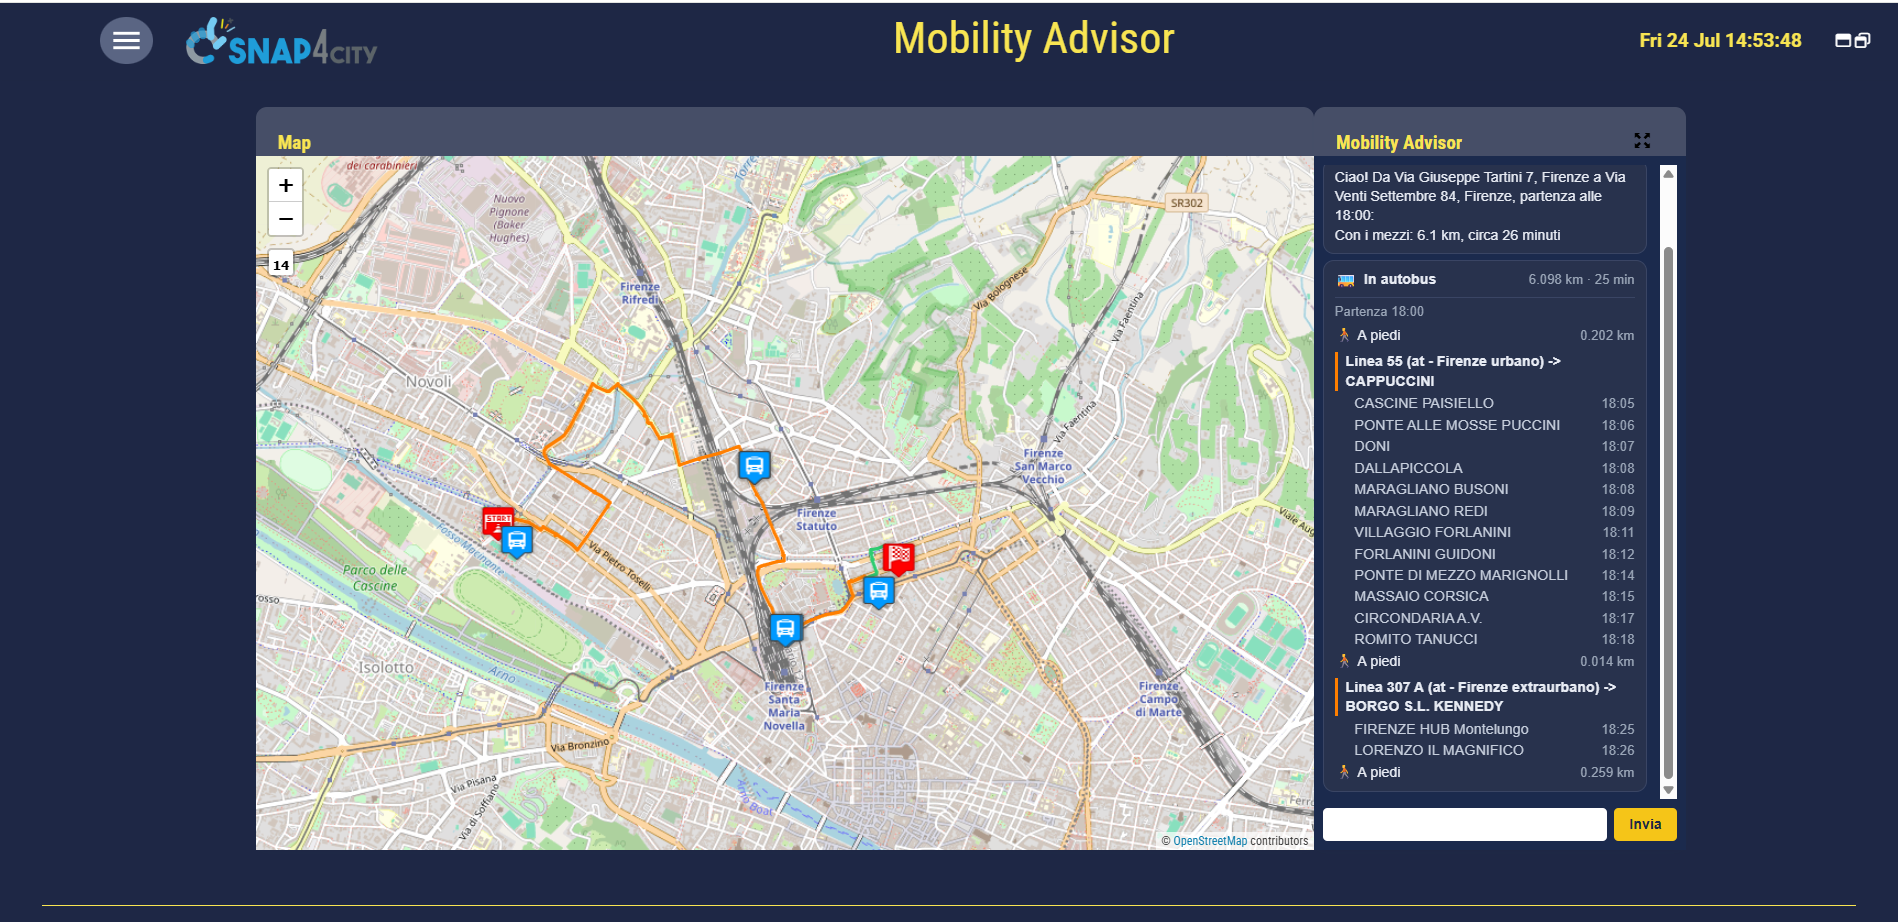
\includegraphics[width=\textwidth]{S19-orario-partenza.jpg}
  \caption{Itinerario di trasporto pubblico con l'orario di partenza indicato.}
  \label{fig:S19}
\end{figure}

\subsection{S20 --- Richiesta non supportata}
\textbf{Situazione.} Le richieste fuori ambito (orari o linee del treno) ricevono una
risposta cortese che indica la funzione non supportata, senza dati geografici.
\textbf{Riproduzione.} L'utente digita \emph{``a che ora passa il treno?''}.
\textbf{Output completo:} \exfile{S20-non-supportato}.
\begin{figure}[htbp]
  \centering
  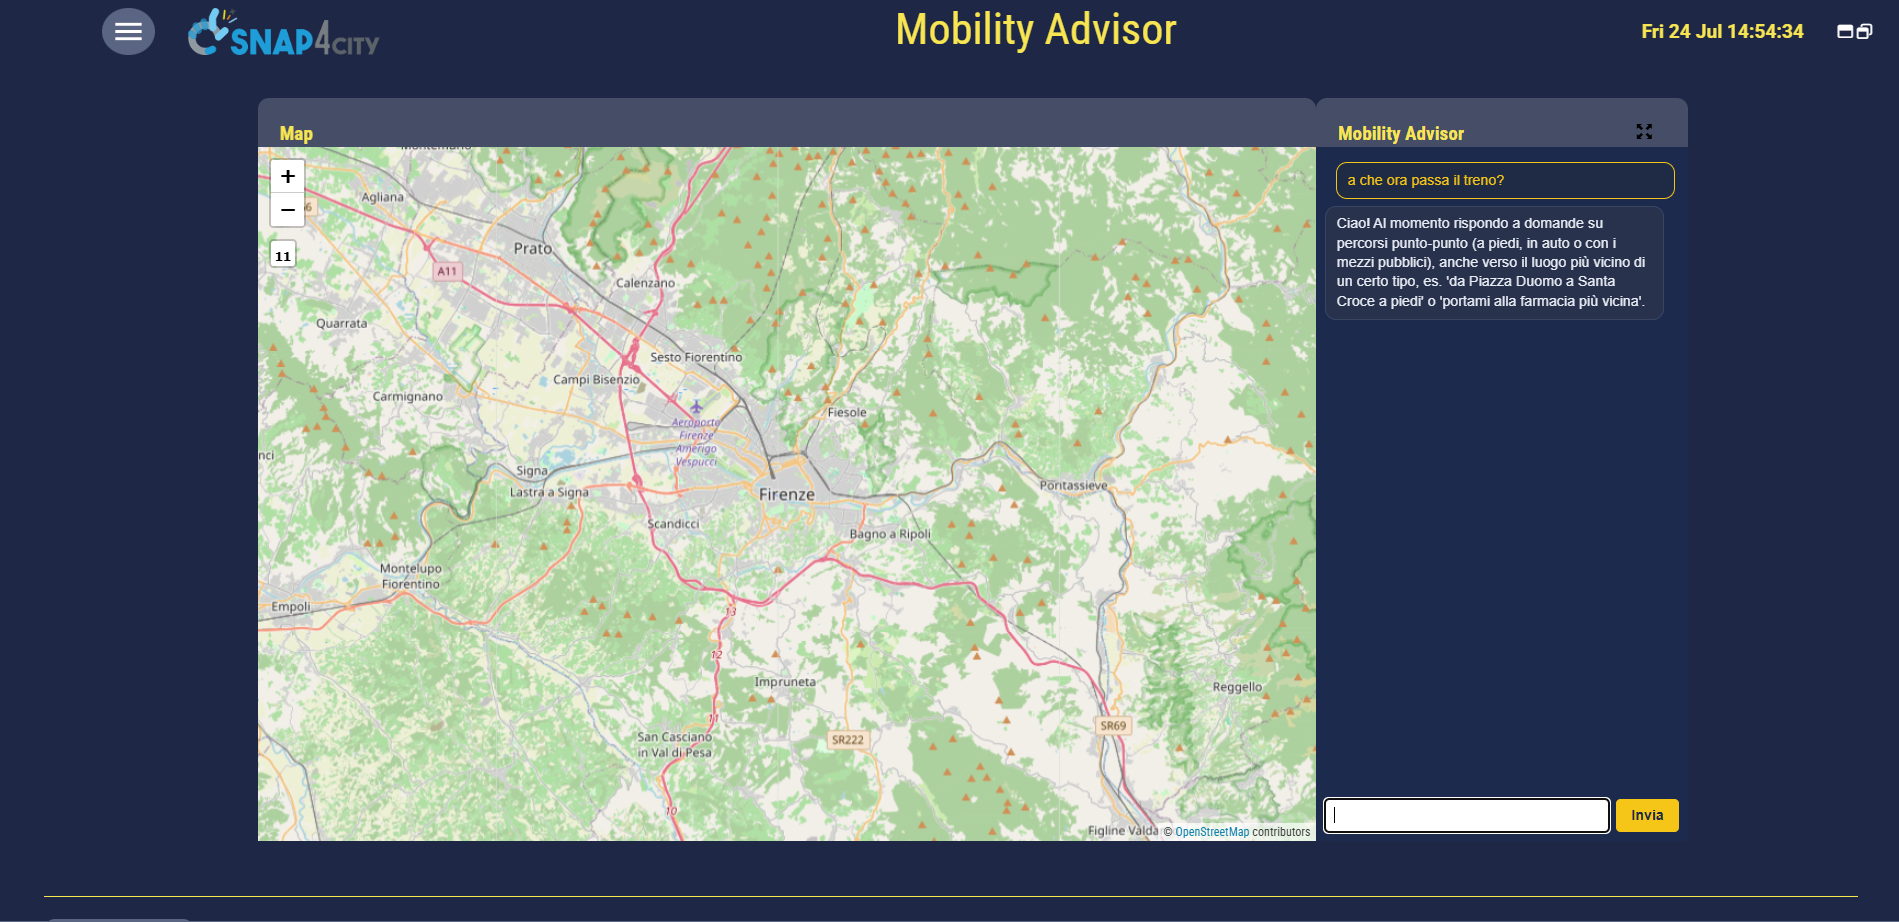
\includegraphics[width=\textwidth]{S20-non-supportato.jpg}
  \caption{Risposta cortese per una richiesta non supportata.}
  \label{fig:S20}
\end{figure}

\subsection{S21 --- Chiarimento di uno slot mancante}
\textbf{Situazione.} Se manca il luogo o la categoria, l'advisor chiede un chiarimento
prima di procedere, senza cancellare la mappa.
\textbf{Riproduzione.} L'utente digita \emph{``mostrami le farmacie''} (senza luogo) oppure
\emph{``cosa c'\`e qui intorno?''} (senza categoria).
\textbf{Output completo:} \exfile{S21-chiarimento}.
\begin{figure}[htbp]
  \centering
  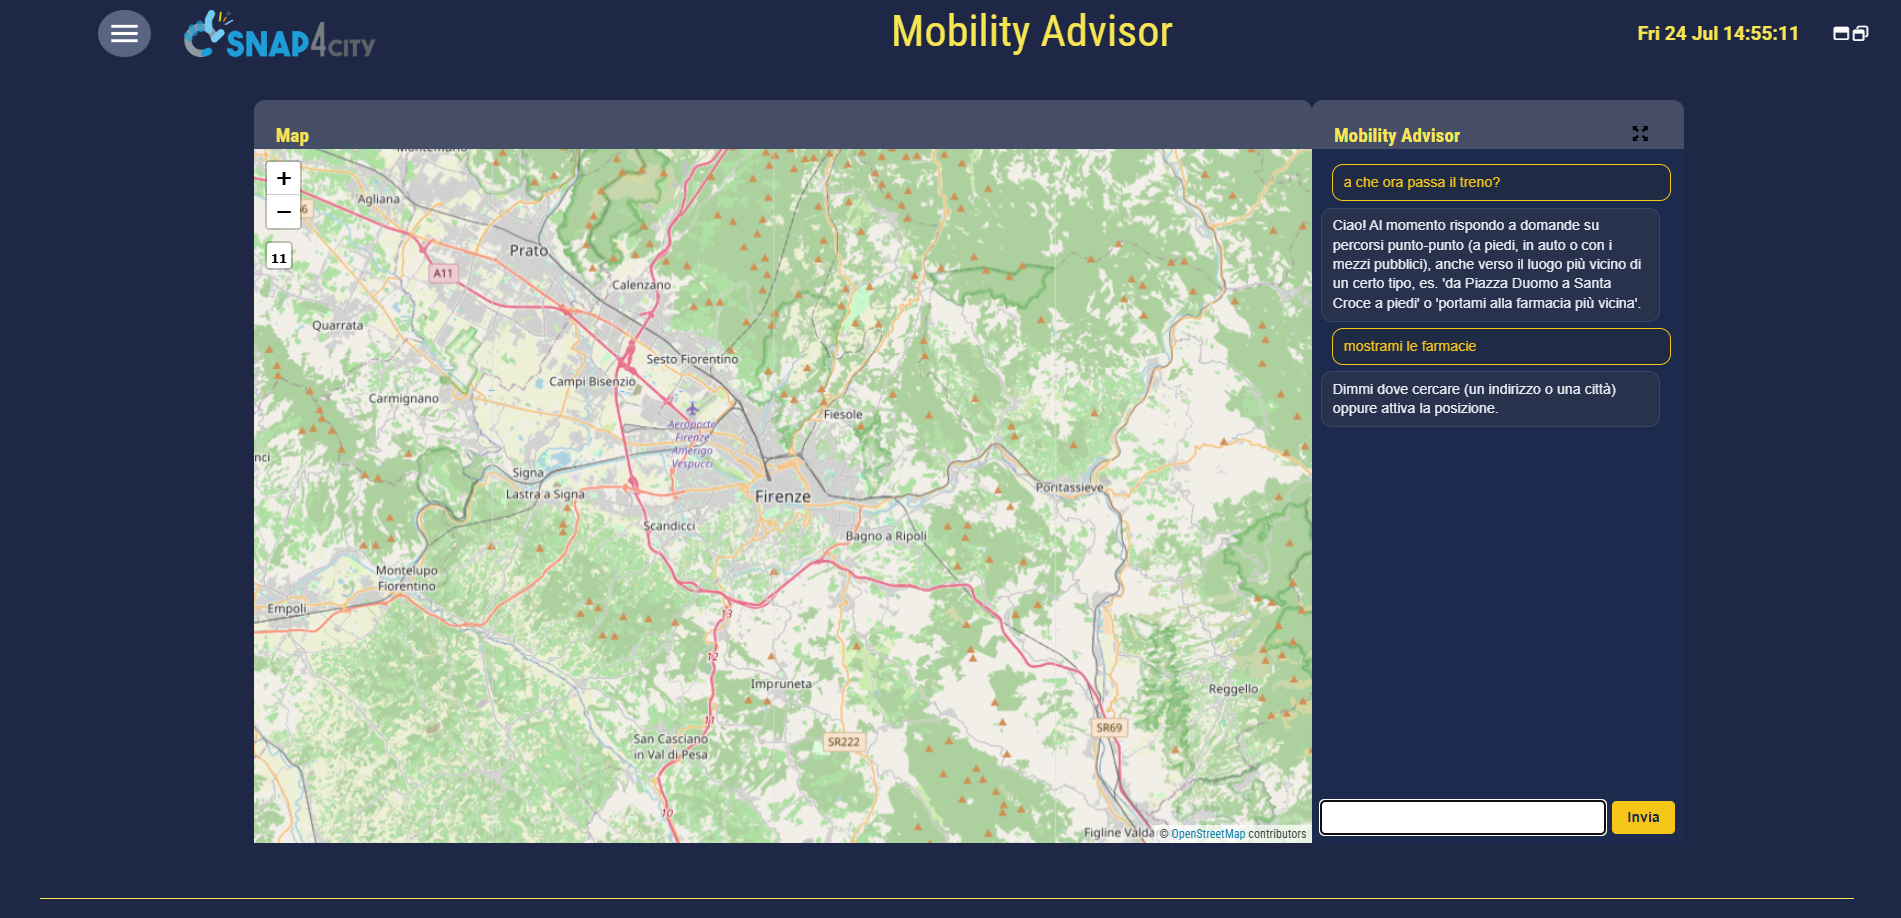
\includegraphics[width=\textwidth]{S21-chiarimento.jpg}
  \caption{Domanda di chiarimento (``dove?'' / ``che tipo?'').}
  \label{fig:S21}
\end{figure}

% =====================================================================
\chapter{Test e validazione}

\section{Suite automatica}

La suite conta \textbf{126 test} eseguibili ovunque: sono completamente \emph{offline}
e non richiedono n\'e il modello n\'e i server MCP. I doppi di test sostituiscono il
client MCP con una coda deterministica di risposte e il client LLM con una risposta
predefinita; la Tabella~\ref{tab:test} ne riassume la composizione.

\begin{table}[htbp]
  \centering
  \small
  \begin{tabular}{lrp{0.48\textwidth}}
    \toprule
    \textbf{File} & \textbf{Test} & \textbf{Copertura} \\
    \midrule
    \texttt{test\_orchestrator.py} & 74 & nodi del grafo, risoluzione degli estremi, concorrenza, composizione della risposta \\
    \texttt{test\_mcp\_server.py}  & 20 & tool \texttt{route}, suddivisione delle tratte, geocodifica \\
    \texttt{test\_mcp\_tools.py}   & 13 & doppia passata, parser degli envelope, riduzione del contesto \\
    \texttt{test\_api.py}          &  9 & sanificazione del GPS e API del bridge \\
    \texttt{test\_gtfs\_shapes.py} &  6 & scelta della variante, taglio della geometria, degradazioni \\
    \texttt{test\_llm.py}          &  4 & ritentativi su errori transitori, credenziali \\
    \bottomrule
  \end{tabular}
  \caption{Composizione della suite di test.}
  \label{tab:test}
\end{table}

\section{Validazione sul campo}

Il sistema \`e stato verificato end-to-end sulla dashboard; il
Capitolo~\ref{cap:casistica} raccoglie gli scenari con le relative schermate e gli output.
La Tabella~\ref{tab:misure} riepiloga alcune misure di turni reali, i cui output completi
sono allegati nella cartella \texttt{examples/}.

\begin{table}[htbp]
  \centering
  \begin{tabular}{llrr}
    \toprule
    \textbf{Scenario} & \textbf{Modo} & \textbf{Distanza} & \textbf{Durata} \\
    \midrule
    S01 --- Tre modi         & auto              & 2,956 km & 0:04:48 \\
                             & trasporto pubblico& 3,595 km & 0:32:47 \\
                             & a piedi           & 3,062 km & 0:36:44 \\
    \midrule
    S08 --- Autobus (modo singolo)           & trasporto pubblico & 3,938 km & 0:20:35 \\
    S14 --- Auto + servizi lungo il percorso & auto               & 5,688 km & 0:08:34 \\
    \bottomrule
  \end{tabular}
  \caption{Misure da turni reali (output completi in \texttt{examples/}).}
  \label{tab:misure}
\end{table}

Nel confronto a tre modi l'auto \`e la pi\`u rapida (e la pi\`u breve in distanza), il
percorso a piedi \`e il pi\`u lento, mentre il trasporto pubblico segue la rete delle
linee --- quindi copre pi\`u strada --- con un tempo intermedio. Sul fronte dei tempi di
risposta, le misure sul router
mostrano una netta asimmetria: i profili \texttt{foot} e \texttt{car} rispondono in
circa 0,3--0,5 secondi, mentre \texttt{bus} richiede 30--45 secondi.

% =====================================================================
\chapter{Conclusioni}

Il lavoro ha prodotto un advisor di mobilit\`a funzionante e integrato nella dashboard
Snap4City, capace di rispondere in linguaggio naturale confrontando percorsi a piedi,
in auto e con il trasporto pubblico, di risolvere destinazioni generiche a partire dalla
posizione dell'utente e di mostrare i servizi lungo il tragitto.

L'architettura scelta --- una sola chiamata al modello linguistico, per l'estrazione dei
parametri, e codice deterministico per l'esecuzione degli strumenti e la formulazione
della risposta --- rende il comportamento del sistema riproducibile e verificabile con
una suite di test interamente offline.

% =====================================================================
\addcontentsline{toc}{chapter}{Bibliografia}
\begin{thebibliography}{9}

\bibitem{mcp}
Anthropic, \emph{Model Context Protocol --- Specification}.
\url{https://modelcontextprotocol.io}

\bibitem{fastmcp}
\emph{FastMCP --- The fast, Pythonic way to build MCP servers and clients}.
\url{https://github.com/jlowin/fastmcp}

\bibitem{langgraph}
LangChain, \emph{LangGraph --- Building stateful, multi-actor applications with LLMs}.
\url{https://langchain-ai.github.io/langgraph/}

\bibitem{snap4city}
DISIT Lab, Universit\`a degli Studi di Firenze, \emph{Snap4City --- Smart aNalytic
APp builder for sentient Cities}. \url{https://www.snap4city.org}

\bibitem{km4city}
DISIT Lab, \emph{Km4City --- Knowledge Model for the City}.
\url{https://www.km4city.org}

\bibitem{graphhopper}
GraphHopper GmbH, \emph{GraphHopper Routing Engine}.
\url{https://www.graphhopper.com}

\bibitem{gtfs}
\emph{General Transit Feed Specification (GTFS) Reference}.
\url{https://gtfs.org/documentation/schedule/reference/}

\end{thebibliography}

\end{document}
